% -*- TeX:SI -*-
% slovene sub-mode for spell check
%%%%%%%%%%%%%%%%%%%%%%%%%%%%%%%%%%%%%%%%%%%%%%%%%%%%%%%%%%%%%%%%%%%%%%%%%%%%%%%%%%%%%%%%%%%%%%%%%%%%%%%%%%%%%%%%%%%%%%%%
% LaTeX predloga za zaključna dela
% Univerza v Ljubljani, Fakulteta za elektrotehniko
% Zbral in uredil: Roman Kamnik, junij 2013
% Dopolnil: Sebastjan Šlajpah (2013), Sašo Tomažič (2013), Peter Miklavčič (2019), Peter Kmecl (2023)
%%%%%%%%%%%%%%%%%%%%%%%%%%%%%%%%%%%%%%%%%%%%%%%%%%%%%%%%%%%%%%%%%%%%%%%%%%%%%%%%%%%%%%%%%%%%%%%%%%%%%%%%%%%%%%%%%%%%%%%%
\documentclass[a4paper,twoside,openright,12pt,slovene]{book}
\usepackage[pdftex]{./Izgled/UNI-LJ-FE-Diploma} % stil zaključnega dela UL FE
\usepackage[utf8]{inputenc} % predloga uporablja standardno kodiranje Unicode UTF-8, ki podpira šumnike
\usepackage[greek,english,slovene]{babel} % seznam uporabljenih jezikov (zadnji na seznamu je primarni)

% PDF/A %%%%%%%%%%%%%%%%%%%%%%%%%%%%%%%%%%%%%%%%%%%%%%%%%%%%%%%%%%%%%%%%%%%%%%%%%%%%%%%%%%%%%%%%%%%%%%%%%%%%%%%%%%%%%%%%
% Več o PDF/A v LaTeX-u: https://www.mathstat.dal.ca/~selinger/pdfa/
\usepackage{filecontents}

\usepackage{svg}
\usepackage{amsmath}
\usepackage{comment}
\begin{filecontents*}[overwrite]{\jobname.xmpdata}
    \Title{Zasnova in izdelava komunikacijskega modula za števec električne energije} % Mora biti enak kot je v prijavi teme!
    \Author{Krištof Frelih} % Mora biti enak kot na naslovnici!
\end{filecontents*}
\usepackage[a-1b]{pdfx}
%%%%%%%%%%%%%%%%%%%%%%%%%%%%%%%%%%%%%%%%%%%%%%%%%%%%%%%%%%%%%%%%%%%%%%%%%%%%%%%%%%%%%%%%%%%%%%%%%%%%%%%%%%%%%%%%%%%%%%%%

% LaTeX PAKETI %%%%%%%%%%%%%%%%%%%%%%%%%%%%%%%%%%%%%%%%%%%%%%%%%%%%%%%%%%%%%%%%%%%%%%%%%%%%%%%%%%%%%%%%%%%%%%%%%%%%%%%%%
% Kompakten pregled LaTeX ukazov je dostopen na https://en.wikibooks.org/wiki/Category:Book:LaTeX
% Navodila posameznih uporabljenih paketov so dostopna na https://www.ctan.org

% Dodatni simboli
\usepackage{textcomp}                               % dodatni simboli (kot npr. €)
\usepackage{gensymb}                                % dodatni simboli \de­gree, \cel­sius, \pert­hou­sand, \mi­cro, \ohm

% Enote in števila
\usepackage{siunitx}
\DeclareSIUnit\bit{bit}
\DeclareSIUnit\baud{baud}
\sisetup{per-mode=symbol}

\sisetup{
  output-decimal-marker = {,},
  input-decimal-markers = {.,,},
}

\newcommand{\uppi}{\textrm{\greektext p\latintext}} % velika grška črka P z \uppi, alternativa simbolu \Pi

% Osnovno oblikovanje
\hypersetup{unicode,hidelinks,breaklinks,hyperindex} % dodatne možnosti hiperpovezav
\usepackage[normalem]{ulem}                          % podčrtavanje in prečrtavanje teksta
\usepackage{float}                                   % dodatne možnosti oblikovanja objektov
\usepackage{enumitem}                                % dodatne možnosti oblikovanja seznamov

% Dodatno oblikovanje
%\zamaknirobsodihstrani{0mm} % dodatna prilagoditev levega roba sodih strani za dvostranski tisk
%\usepackage{dcolumn}        % poravnava po decimalnih mestih v tabelah
\usepackage{longtable}      % večstranske tabele
%\usepackage{caption}        % dodatne možnosti označevanja objektov
%\usepackage{rotating}       % vretenje objektov, strani, ipd.

% Matematična orodja
\usepackage{mathtools} % http://mirrors.ctan.org/macros/LaTeX/contrib/mathtools/mathtools.pdf
\usepackage{bm}        % ukaz za odebeljeni tisk \bm v matematičnih okoljih
%\usepackage{cancel}   % ukaz za prečrtavanje \cancel v matematičnih okoljih

% Grafična orodja
\usepackage{graphicx}                 % vključevanje bitnih slik z ukazom \includegraphics
\usepackage{grffile}                  % podpora presledkom pri ukazu \includegraphics
%\usepackage{tikz}                    % paket TikZ za risanje (npr. blokovnih shem, diagramov poteka, itd.)
%\usetikzlibrary{calc,shapes,arrows}  % dodatne možnosti paketa TikZ
%\usepackage{tikzscale}               % skaliranje risb
%\usepackage[smartlabels]{circuitikz} % risanje shem vezij
%\usepackage{pgfplots}                % paket PGFPlots za risanje grafov, tudi iz CSV in podobnih datotek
%\usepgfplotslibrary{polar,external}  % dodatne možnosti paketa PGFPlots
%\usepackage{tikz-3dplot}             % 3D risanje
% Primeri: http://texample.net , http://pgfplots.net/tikz/examples , http://pgfplots.sourceforge.net/gallery.html

% Vključevanje datotek
\usepackage{pdfpages} % vključevanje PDF datotek z ukazom \includegraphics
\usepackage{epstopdf} % vključevanje EPS datotek z ukazom \includegraphics
\usepackage{listings} % orodja za izpisovanje programske kode
\lstset{              % nastavitve orodja za izpisovanje programske kode
    basicstyle=\ttfamily\footnotesize,
    breaklines=true,
    numbers=left,
    numberstyle=\scriptsize,
    keywordstyle=\color{blue},
    commentstyle=\color{unilj},
    stringstyle=\color{olive},
}
%%%%%%%%%%%%%%%%%%%%%%%%%%%%%%%%%%%%%%%%%%%%%%%%%%%%%%%%%%%%%%%%%%%%%%%%%%%%%%%%%%%%%%%%%%%%%%%%%%%%%%%%%%%%%%%%%%%%%%%%

% DEKLARACIJE %%%%%%%%%%%%%%%%%%%%%%%%%%%%%%%%%%%%%%%%%%%%%%%%%%%%%%%%%%%%%%%%%%%%%%%%%%%%%%%%%%%%%%%%%%%%%%%%%%%%%%%%%%
\naslov{Zasnova in izdelava komunikacijskega modula za števec električne energije} % Mora biti enak kot je v prijavi teme!
\avtor{Krištof Frelih} % Mora se ujemati s \Title pri metapodatkih PDF/A!
\mentor{prof. dr. Andrej Žemva}
%\somentor{Naziv, ime in priimek somentorja}
\date{Ljubljana, \the\year}
\univerza{Univerza v Ljubljani}
\definecolor{unilj}{cmyk}{0.00, 0.94, 0.94, 0.06} % barva Univerze v Ljubljani

% Potrebno je paziti, da je izbrana prava kombinacija tipa dela in sodelujočih fakultet glede na študijski program!
%\delo{Diplomsko delo\\~\\Univerzitetni študijski program prve stopnje Elektrotehnika}
%\delo{Diplomsko delo\\~\\Univerzitetni študijski program prve stopnje Multimedija}
%\delo{Diplomsko delo\\~\\Visokošolski strokovni študijski program\\prve stopnje Aplikativna elektrotehnika}
%\delo{Diplomsko delo\\~\\Visokošolski strokovni študijski program\\prve stopnje Multimedijske komunikacije}
\delo{Magistrsko delo\\~\\Magistrski študijski program druge stopnje Elektrotehnika}
%\delo{Magistrsko delo\\~\\Magistrski študijski program druge stopnje Uporabna statistika}
\fakulteta{Fakulteta za elektrotehniko}
%\fakulteta{Fakulteta za elektrotehniko,\\Fakulteta za računalništvo in informatiko} % Za program Multimedija
%\fakulteta{Fakulteta za elektrotehniko, Biotehniška fakulteta,\\Ekonomska fakulteta, Fakulteta za družbene vede,\\Fakulteta za matematiko in fiziko, Fakulteta za\\računalništvo in informatiko, Medicinska fakulteta} % Za program Uporabna statistika
%%%%%%%%%%%%%%%%%%%%%%%%%%%%%%%%%%%%%%%%%%%%%%%%%%%%%%%%%%%%%%%%%%%%%%%%%%%%%%%%%%%%%%%%%%%%%%%%%%%%%%%%%%%%%%%%%%%%%%%%

% DOKUMENT %%%%%%%%%%%%%%%%%%%%%%%%%%%%%%%%%%%%%%%%%%%%%%%%%%%%%%%%%%%%%%%%%%%%%%%%%%%%%%%%%%%%%%%%%%%%%%%%%%%%%%%%%%%%%
\begin{document}
\frontmatter

\selectlanguage{slovene}

%******************************* NASLOVNICA ************************************
\maketitle

%******************************* ZAHVALA ***************************************
\zahvala
Najprej bi se rad zahvalil mentorju, prof.~dr.~Andreju Žemvi, za odzivnost in pomoč pri pisanju magistrskega dela.

Zahvaljujem se podjetju Iskraemeco d.d. in vsem sodelavcem za vse spodbudne, strokovne in manj strokovne pogovore na delovnem mestu ... ali pa pred kavomatom.

Zahvala gre moji družini in vsem prijateljem, s katerimi sem užival čas med vožnjami v Ljubljano, ob skupnem učenju, prijetnih druženjih med odmori in iskal ravnotežje v plezališčih ali pa se v hribih, navezan na vrv, oziral za zahajajočim soncem. Prav vsak od vas je zaslužen, da sem študij pripeljal do konca.

Najlepša zahvala pa gre ženi Katarini za vse spodbude, potrpežljivost in pomoč med študijem.

%******************************* POVZETEK IN KLJUČNE BESEDE ********************
\povzetek
V magistrskem delu smo obravnavali razvoj in razvojno testiranje komunikacijskega modula za družino pametnih števcev električne energije IE.X podjetja Iskraemeco d.d. 
\par Komunikacijski moduli omogočajo brezžično odčitavanje in parametriranje pametnega števca električne energije prek mobilnih omrežij. Zasnovani so kot ločena, izmenljiva enota števca, kar omogoča prilagoditev komunikacijske tehnologije zahtevam posameznega trga brez posega v sam števec.
\par Uvodoma smo predstavili pametni števec in vlogo mobilnih omrežij pri daljinskem odčitavanju ter primerjali mobilne tehnologije, ki jih podjetje uporablja. Izhajajoč iz zahtev internega standarda P* smo določili električne in mehanske lastnosti komunikacijskega modula ter opisali razvoj njegovih glavnih funkcijskih sklopov. Nato smo predstavili razvojno testiranje modula, v okviru katerega smo avtomatizirali postopek za testiranje funkcije varnega ugašanja modula in na podlagi rezultatov predlagali možnosti za nadaljnje izboljšave.

\kljucnebesede
pametni števec, komunikacijski modul, LTE Cat-M, NB-IoT, antena

\selectlanguage{english}

%******************************* ABSTRACT AND KEYWORDS *************************

\abstract In this master's thesis we addressed the development and development testing of a communication module for the IE.X family of smart electricity meters manufactured by Iskraemeco d.d.
\par Communication modules enable wireless remote reading and parameterization of a smart electricity meter over mobile networks. They are designed as a separate, interchangeable unit of the meter, which allows the communication technology to be adapted to the requirements of an individual market without any intervention in the meter itself.
\par We first presented the smart meter and the role of mobile networks in remote reading, and compared the mobile technologies used by the company. Based on the requirements of the internal P* standard, we determined the electrical and mechanical properties of the communication module and described the development of its main functional blocks. We then presented the development testing of the module, in the course of which we automated the procedure for testing the module's safe shutdown function and, based on the results, proposed options for further improvements.

\keywords
smart meter, communication module, LTE Cat-M, NB-IoT, antenna

\selectlanguage{slovene}

%******************************* KAZALO ****************************************
\tableofcontents

%******************************* SEZNAM SLIK, SEZNAM TABEL *********************
\seznamslik
\seznamtabel

%******************************* SEZNAM SIMBOLOV *******************************
\seznamsimbolov
V pričujočem zaključnem delu so uporabljene naslednje veličine in simboli:

\begin{center}
    \begin{tabular}{*{4}{l}} \hline
        \multicolumn{2}{c}{\bf{Veličina / oznaka}} & \multicolumn{2}{c}{\bf{Enota}} \\ \hline
        Ime & Simbol & Ime & Simbol \\ \hline
        čas & $t$ & sekunda & s \\
        frekvenca & $f$ & hertz & Hz \\
        napetost & $U$ & volt & V \\
        tok & $I$ & ampere & A \\
        upornost & $R$ & ohm & $\Omega$ \\
        kapacitivnost & $C$ & farad & F \\
        moč & $P$ & watt & W \\
        koeficient odboja & $\Gamma$ & -- & -- \\
        razmerje stoječega vala & $\mathrm{SWR}$ & -- & -- \\
        povratno slabljenje & $\mathrm{Return\ Loss}$ & decibel & dB \\
        S11 & $S_{11}$ & decibel & dB \\


    \end{tabular}
\end{center}

\seznamkratic
V pričujočem zaključnem delu so uporabljene naslednje kratice:

\begin{center}
    \begin{longtable}{p{2.5cm}|p{5.75cm}|p{5.75cm}} \hline %Dolga tabela kratic (večstranska)
        Kratica & Pomen v slovenščini & Pomen v angleščini \\ \hline\endhead %Glava, ki se ponovi na začetku vsake strani tabele
        \hline\endfoot %Zaključek tabele na vsaki strani
        %Začetek vsebine tabele
2FF    & format kartice SIM (mini-SIM) & 2FF SIM card form factor (mini-SIM) \\
3GPP   & partnerski projekt za standardizacijo 3. generacije & 3rd Generation Partnership Project \\
8PSK   & 8-fazna modulacija s premikom faze & 8 Phase Shift Keying \\
AMI    & napredna merilna infrastruktura & Advanced Metering Infrastructure \\
AMR    & samodejno odčitavanje števcev & Automated Meter Reading \\
APN    & ime dostopne točke & Access Point Name \\
ARFCN  & absolutna številka radijskega frekvenčnega kanala & Absolute Radio Frequency Channel Number \\
AT     & ukazni nabor AT & AT Commands \\
BER    & razmerje bitnih napak & Bit Error Rate \\
CMUX   & protokol za multipleksiranje kanalov & Multiplexer protocol \\
CTS    & potrditev za pošiljanje & Clear To Send \\
DLCI   & identifikator povezave podatkovnega sloja & Data Link Connection Identifier \\
DFOTA  & diferencialna posodobitev vgrajene programske opreme na daljavo & Delta Firmware Over-The-Air \\
EDGE   & nadgradnja GPRS (2.75G) & Enhanced Data rates for GSM Evolution \\
EDLC   & kondenzator z elektrostatičnim dvojnim slojem & Electric Double-Layer Capacitor \\
EMC    & elektromagnetna združljivost & Electromagnetic Compatibility \\
EMI    & elektromagnetne motnje & Electromagnetic Interference \\
ESD    & elektrostatična razelektritev & Electrostatic Discharge \\
ESR    & ekvivalentna serijska upornost & Equivalent Series Resistance \\
ETSI   & Evropski inštitut za telekomunikacijske standarde & European Telecommunications Standards Institute \\
eSIM   & vgrajena kartica SIM & embedded SIM \\
FDD    & frekvenčni dupleks & Frequency Division Duplex \\
FEM    & zamenljivi funkcijski modul & Field Exchangeable Module \\
FOTA   & posodobitev vgrajene programske opreme na daljavo & Firmware Over-The-Air \\
G3-PLC & komunikacija po elektroenergetskem omrežju G3 & G3 Power Line Communication \\
GMSK   & Gaussova modulacija s premikom frekvence & Gaussian Minimum Shift Keying \\
GPIO   & splošnonamenski vhod/izhod & General-Purpose Input/Output \\
GPRS   & paketna radijska storitev v omrežjih GSM & General Packet Radio Service \\
GSM    & globalni sistem za mobilne komunikacije & Global System for Mobile Communications \\
HSPA   & paketni dostop z visoko hitrostjo & High Speed Packet Access \\
IP     & internetni protokol & Internet Protocol \\
IPv4   & internetni protokol, različica 4 & Internet Protocol version 4 \\
IPv6   & internetni protokol, različica 6 & Internet Protocol version 6 \\
IoT    & internet stvari & Internet of Things \\
LCD    & zaslon s tekočimi kristali & Liquid Crystal Display \\
LGA    & ohišje tipa LGA & Land Grid Array \\
LPWA   & širokopodročno omrežje z majhno porabo energije & Low-Power Wide-Area \\
LTE    & dolgoročna evolucija (mobilno omrežje 4G) & Long Term Evolution \\
LTE-M  & LTE za stroje (LTE Cat-M1) & LTE for Machines (LTE Cat-M1) \\
M-Bus  & komunikacijsko vodilo Meter-Bus & Meter-Bus \\
M2M    & komunikacija stroj--stroj & Machine-to-Machine \\
MFF2   & format kartice eSIM (MFF2) & MFF2 SIM form factor \\
NB-IoT & ozkopasovni internet stvari & Narrowband Internet of Things \\
NMOS   & N-kanalni MOSFET & N-channel Metal-Oxide-Semiconductor Field-Effect Transistor \\
NN     & nizkonapetostno (omrežje) & low-voltage (network) \\
OFDMA  & večkratni dostop z ortogonalnim frekvenčnim multipleksiranjem & Orthogonal Frequency-Division Multiple Access \\
OTA    & brezžični prenos podatkov & Over-The-Air \\
PCB    & tiskano vezje & Printed Circuit Board \\
PDP    & paketni podatkovni protokol & Packet Data Protocol \\
PMOS   & P-kanalni MOSFET & P-channel Metal-Oxide-Semiconductor Field-Effect Transistor \\
PPP    & protokol točka--točka & Point-to-Point Protocol \\
RS-485 & serijski komunikacijski standard RS-485 & RS-485 Serial Communication Standard \\
RTS    & zahteva za pošiljanje & Request To Send \\
SC-FDMA & enonosilčni FDMA & Single-Carrier Frequency Division Multiple Access \\
SIM    & naročniški identifikacijski modul & Subscriber Identity Module \\
SISO   & en vhod, en izhod & Single-Input Single-Output \\
SMD    & površinsko montirana komponenta & Surface-Mount Device \\
SWR    & razmerje stoječega vala & Standing Wave Ratio \\
TDMA   & časovni večkratni dostop & Time Division Multiple Access \\
TIS    & skupna izotropna občutljivost & Total Isotropic Sensitivity \\
TRP    & skupna izsevana moč & Total Radiated Power \\
TX     & oddajanje & transmit \\
UART   & univerzalni asinhroni oddajnik/sprejemnik & Universal Asynchronous Receiver/Transmitter \\
UMTS   & univerzalni mobilni telekomunikacijski sistem & Universal Mobile Telecommunications System \\
USB    & univerzalno serijsko vodilo & Universal Serial Bus \\
VNA    & vektorski analizator omrežij & Vector Network Analyzer \\
VSWR   & napetostno razmerje stoječega vala & Voltage Standing Wave Ratio \\
wM-Bus & brezžični Meter-Bus & Wireless Meter-Bus \\

        %konec vsebine tabele
    \end{longtable}
\end{center}



\mainmatter

%******************************* UVOD ******************************************
\chapter{Uvod} \label{uvod}

Magistrsko delo je nastalo v sodelovanju s podjetjem Iskraemeco~d.d., v oddelku
Razvoj in raziskave, ki se ukvarja z razvojem pametnih števcev električne energije
(angl. smart energy meter) in njihovih izmenljivih modulov.
Pametni števci imajo poleg funkcij za merjenje električne energije tudi vlogo zbiranja in pošiljanja podatkov iz drugih merilnih naprav v gospodinjstvu (npr. vodni števec, kalorimeter, števec plina) \cite{skalar_zasnova_nodate}. V večini primerov podatke iz drugih merilnih naprav zbirajo prek lokalnih žičnih in brezžičnih omrežij (M-Bus, wM-Bus, RS-485), agregirane podatke pa nato pošljejo naprej prek komunikacije po elektroenergetskem omrežju (G3-PLC) ali prek mobilnega omrežja (npr. GPRS, LTE-M, NB-IoT), kot to prikazuje slika \ref{fig:AMI arhitektura}. 

\begin{figure}[h]
    \centering
    \includesvg[
    width=0.8\columnwidth,inkscapelatex=false
    ]{Slike/AMI.drawio.svg}
    \caption{\label{fig:AMI arhitektura} Pametni števec kot zbirna točka podatkov merilnikov komunalnih storitev}
\end{figure}
\newpage
Večina pametnih števcev družine IE.X podjetja Iskraemeco d.d. ima modularno zasnovo, ki omogoča zamenjavo komunikacijskega modula tudi po tem, ko je števec že nameščen pri končnem uporabniku. To kasneje v življenjski dobi števca omogoča nadgradnjo komunikacijskega modula in zamenjavo mobilnega omrežja, lahko pa se distribucija že v začetku izvedbe projekta odloči za več tehnologij odčitavanja števca \cite{Croatia}. Poenostavljeno arhitekturo pametnega števca prikazuje slika \ref{blok_shema_stevec}.

\begin{figure}[h]
    \centering
    \includesvg[
    width=0.8\columnwidth,inkscapelatex=false
    ]{Slike/blok_shema_stevc.svg}
    \caption{\label{blok_shema_stevec} Poenostavljena arhitektura pametnega števca}
\end{figure}
\par Cilj magistrskega dela je razvoj in razvojno testiranje komunikacijskega modula za družino pametnih števcev IE.X podjetja Iskraemeco d.d.

%prestavimo spodnjo stvar nižje
\begin{comment}
Komunikacijski modem števcu omogoča naslednje funkcije:
\begin{itemize}[noitemsep]
    \item daljinsko odčitavanje in parametriranje,
    \item možnost oddaljene posodobitve  delov vgrajene programske opreme (DFOTA),
    \item obveščanje električne distribucije o dogodkih in izpadih na NN omrežju (funkcija last gasp),

\end{itemize}
\end{comment}

%******************************* POGLAVJA **************************************

\chapter{Primerjava mobilnih omrežij za odčitavanje števcev} \label{Primerjava mobilnih omrežij za odčitavanje števcev}
    Mobilna omrežja predstavljajo pomemben komunikacijski medij za daljinsko odčitavanje števcev in prenos merilnih podatkov v naprednih merilnih sistemih (AMI). Leta 1988 je Iskraemeco predstavil prvi elektronski sistem za samodejno odčitavanje števcev (AMR), leta 1998 pa prvi rezidenčni AMR sistem za gospodinjske uporabnike \cite{Iskraemeco_80_let}. Števec MT372, ki je omogočal prenos podatkov po omrežju 2G, je bil razvit leta 2005.
    Za odčitavanje števcev se v Iskraemecu uporablja več različnih mobilnih omrežnih tehnologij. Časovni razvoj in razdelitev mobilnih omrežij po generacijah prikazuje slika \ref{omrezje}.
    
    \begin{figure}[H]
    \centering
    \includesvg[width=0.7\columnwidth]{Slike/omrezja.svg}
    \caption{\label{omrezje} Pregled mobilnih omrežij po generacijah \cite{omrezja}}
    \end{figure}

\section{Omrežja druge generacije} \label{2G}

Omrežja druge generacije (2G) temeljijo na sistemu GSM, ki je bil prvič implementiran leta 1991 kot vodovno komutirano omrežje, primarno namenjeno glasovni telefoniji. Frekvenčni spekter danes še vedno uporabljenega sistema GSM je razdeljen na \SI{25}{\mega\hertz} široke pasove \cite{GPRS}, pri čemer je vsak pas nadalje razdeljen na 125 kanalov s pasovno širino \SI{200}{\kilo\hertz}. Frekvenčne pasove v omrežjih druge generacije, ki so v uporabi v Evropi, prikazuje tabela \ref{tab:gsm_bands}. Kanali so označeni z identifikacijsko številko ARFCN. Dodatno je v uporabi še časovni sodostop (TDMA), ki vsak posamezen frekvenčni kanal razdeli na osem časovnih rež, uporabljena modulacijska tehnika pa je GMSK. Nazivna hitrost prenosa podatkov v osnovnem sistemu GSM znaša \SI{9,6}{\kilo\bit\per\second}.

\begin{footnotesize}
\begin{table}[H]
    \centering
    \caption{\label{tab:gsm_bands} Frekvenčni pasovi GSM, uporabljeni v Evropi}
    ~\\*
    \begin{tabular}{cccc}
        \hline
        \rule{0pt}{3ex}
        \textbf{Pas GSM} &
        \textbf{Uplink} &
        \textbf{Downlink} &
        \textbf{ARFCN} \\
        \textbf{} &
        \textbf{[MHz]} &
        \textbf{[MHz]} &
        \textbf{} \\[0.5ex]
        \hline
        GSM850         & 824--849   & 869--894   & 128--251 \\
        GSM900 (P-GSM) & 890--915   & 935--960   & 1--124 \\
        GSM900 (E-GSM) & 880--915   & 925--960   & 975--1023, 0--124 \\
        GSM900 (R-GSM) & 876--880   & 921--925   & 940--974, 0--124 \\
        DCS1800        & 1710--1785 & 1805--1880 & 512--885 \\
        \hline
    \end{tabular}
\end{table}
\end{footnotesize}

Sistem GPRS (t. i. 2.5G) je bil razvit kot nadgradnja GSM, pri čemer uvaja paketno komutirano prenosno tehniko namesto izključno vodovno komutirane. Glede na uporabljeni kodni način in razpoložljivo število časovnih rež znaša hitrost prenosa podatkov med približno \SI{56}{\kilo\bit\per\second} in \SI{114}{\kilo\bit\per\second} \cite{ETSI_TS_101_350}.
\newpage
Tehnologija EDGE (t. i. 2.75G) predstavlja nadaljnjo nadgradnjo GPRS. Poleg modulacije GMSK uporablja še modulacijsko shemo 8PSK, kar omogoča bistveno večjo podatkovno prepustnost. Največja teoretična hitrost prenosa podatkov lahko doseže do \SI{473,6}{\kilo\bit\per\second}, pri čemer se še vedno uporablja isti frekvenčni spekter kot v sistemih GSM in GPRS \cite{GPRS}. Omrežja druge generacije se zaradi svoje razširjenosti in dobre pokritosti pogosto uporabljajo kot nadomestna (fallback) komunikacijska tehnologija. 
\section{Omrežja tretje generacije} \label{sec:3g}
    Omrežja tretje generacije so bila uvedena s tehnologijo UMTS (Release 99), ki med drugim namesto kombinacije TDMA in FDMA uporablja sodostop WCDMA, zaradi česar se tudi pasovna širina kanala poveča na \SI{5}{\mega\hertz}. Kasneje sta se razvila še HSDPA in HSUPA, ki sta skupaj tvorila tehnologijo HSPA, pozneje nadgrajeno v HSPA+ (Release 7). Večina evropskih in slovenskih operaterjev je omrežja tretje generacije opustila zaradi potreb po frekvenčnem spektru za nadaljnji razvoj omrežja 4G in 5G \cite{3Gupokojitev}.
    
\section{Omrežja četrte generacije} \label{sec:4g}
    Organizacija 3GPP je LTE razvila kot naslednika omrežij UMTS in HSPA v okviru specifikacij Release~8 (2008). Za večkratni dostop uporablja OFDMA v smeri proti uporabniku in SC-FDMA v smeri od uporabnika. Promet v LTE poteka izključno paketno prek protokola IP. Podpira več pasovnih širin, od \SIrange{1,4}{20}{\mega\hertz}, v konfiguraciji SISO je teoretična največja hitrost prenosa pri \SI{20}{\mega\hertz} do \SI{100}{\mega\bit\per\second} v smeri proti uporabniku in do \SI{50}{\mega\bit\per\second} v smeri od uporabnika. Frekvenčne pasove 4G omrežij prikazuje tabela \ref{tab:lte_bands}.

    Iz LTE sta se kasneje razvila LTE Cat~1, namenjen napravam, ki ne potrebujejo velikih hitrosti prenosa podatkov, in (z Release~13) LTE Cat~1bis, ki dodatno poenostavi strojno opremo zaradi uporabe ene antene namesto dveh, predpisanih pri LTE Cat~1 \cite{ETSI_TS_136_306_V13.5}. LTE-M (LTE Cat-M1) je bil predstavljen v izdaji Release 12 kot standard LPWA, namenjen predvsem IoT- in M2M-povezavam ter baterijsko napajanim napravam \cite{LTE-M}. Pasovna širina je \SI{1,4}{\mega\hertz}, hitrost prenosa podatkov pa do približno \SI{1}{\mega\bit\per\second}.

    V Release~13 je opisan Narrowband Internet of Things (NB-IoT), ki omogoča še nižjo porabo energije in večjo prodornost, vendar v zameno za počasnejši prenos podatkov in daljše zakasnitve \cite{NBIoT}. Za odčitavanje in parametriranje pametnega števca se je po izkušnjah bolje izkazal LTE Cat-M1, saj zaradi višje hitrosti prenosa podatkov olajša nadgradnjo vdelane programske opreme (FOTA) ter branje večje količine podatkov \cite{Trendi_komunikacijskih_tehnologij}. Poleg tega je LTE Cat-M1 primernejši z vidika menjave operaterja in uporabe kartice eSIM namesto klasične kartice SIM.
\begin{footnotesize}
\begin{table}[h]
    \centering
    \caption{\label{tab:lte_bands} Najpogosteje uporabljeni frekvenčni pasovi LTE v Evropi}
    ~\\*
    \begin{tabular}{cccc} \hline
        \rule{0pt}{3ex}
        \textbf{Pas LTE} &
        \textbf{Uplink} &
        \textbf{Downlink} &
        \textbf{Bandwidth} \\
        \textbf{} &
        \textbf{[MHz]} &
        \textbf{[MHz]} &
        \textbf{[MHz]} \\[0.5ex]
        \hline
        1  & 1920--1980 & 2110--2170 & 60 \\
        3  & 1710--1785 & 1805--1880 & 75 \\
        7  & 2500--2570 & 2620--2690 & 70 \\
        8  & 880--915   & 925--960   & 35 \\
        20 & 832--862   & 791--821   & 30 \\
        28 & 703--748   & 758--803   & 45 \\ \hline
    \end{tabular}
\end{table}
\end{footnotesize}
    
\chapter{Potek načrtovanja in razvoja komunikacijskega modula} \label{Potek načrtovanja in razvoja komunikacijskega modula}
Komunikacijski moduli podjetja Iskraemeco so lahko uporabljeni na enofaznih, trifaznih ali indirektnih števcih, zato mora biti modul kompatibilen z že razvitimi števci. Interni standard Iskraemeca P\textsuperscript{*} predpisuje dimenzije modula, glavne električne lastnosti modula, signale med modulom in števcem, njihovo časovno odvisnost ter osnovne ukaze AT. V tem poglavju smo opisali osnovne zahteve za razvoj komunikacijskega modula in razložili delovanje nekaterih funkcij, ki jih modul opravlja.

Števec električne energije ima na svojem zgornjem levem robu priključek FEM (Field Exchangeable Module). Na ta konektor se pritrdi komunikacijski modul. Zaradi morebitne menjave modula ali menjave kartice SIM se lahko modul kadarkoli med delovanjem števca odstrani oziroma vgradi nazaj, ne da bi to kakorkoli vplivalo na delovanje števca. Števec odstranitev modula zazna in dogodek zapiše v svoj dnevnik, saj gre lahko za poskus manipulacije števca. Vgrajen modul prikazuje slika \ref{modul_v_stevcu}.

\begin{figure}[h]
    \centering
    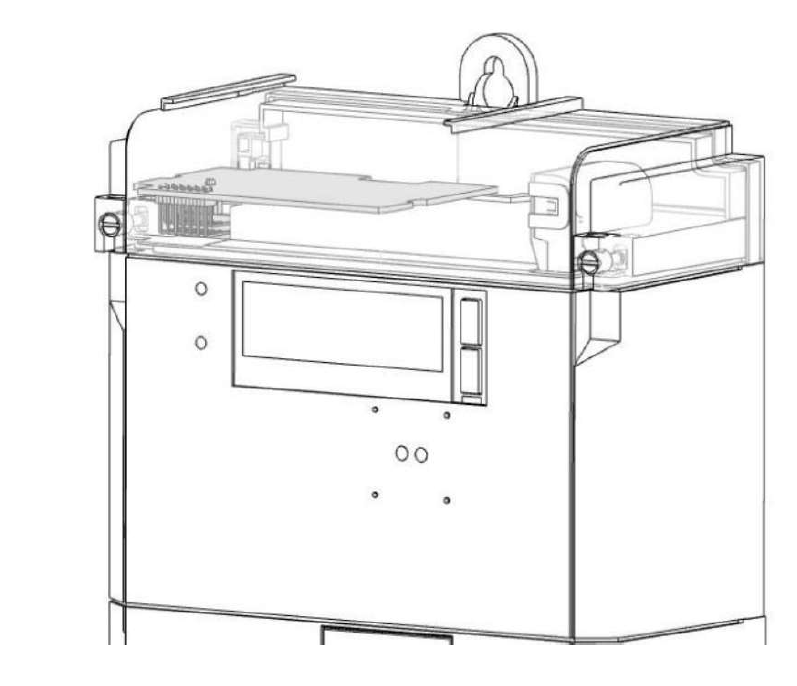
\includegraphics[width=0.6\columnwidth]{Slike/modul_v_stevcu.PNG}
    \caption{\label{modul_v_stevcu} Lokacija komunikacijskega modula v pametnem števcu}
\end{figure}
\section{Zahteve za komunikacijski modul}
Komunikacija med števcem in modulom naj poteka prek vmesnika UART s hitrostjo \SI{115200}{\baud}, 8 podatkovnimi biti in enim stop bitom (115200 8N1) brez strojnega krmiljenja pretoka (angl. hardware flow control). Podpirati mora tudi vmesnik UART za razhroščevanje, prek katerega omogoča nalaganje vgrajene programske opreme s hitrostjo do \SI{3}{\mega\baud} z opcijskim strojnim krmiljenjem pretoka, določene ukaze ter povezavo USB za dodatne možnosti razvoja in razhroščevanja. Največji tok, ki lahko iz števca steče v modul prek konektorja FEM, je \SI{1}{\ampere}, vsa komunikacija s števcem pa je na \SI{3,3}{\volt} napetostnem nivoju. Modul mora vzdržati nenapovedano odstranitev iz števca oziroma odklop napajanja ter podpirati tehnologije LTE Cat-M in NB-IoT s preklopom na GPRS v primeru nedosegljivosti teh omrežij. Z variantno opremljenostjo naj omogoča klasično izmenljivo kartico SIM v formatu 2FF ali kartico eSIM v formatu MFF2. Frekvenčni pasovi, ki naj jih modul podpira, so navedeni v tabeli \ref{tab:bg955_bands}. Na koncu razvoja mora v kombinaciji s števcem ustrezno prestati vse validacijske funkcijske teste, testiranje EMC ter dosegati s standardom predpisane vrednosti TRP in TIS. Izdelava in testiranje modula naj bosta čim bolj enostavna.
Na podlagi zahtev smo izdelali blokovni diagram komunikacijskega modula, ki ga prikazuje slika \ref{fig:blok diagram modula}.
\begin{figure}[h]
    \centering
    \includesvg[inkscapelatex=false, width=0.8\columnwidth]{Slike/blok diagram modula.svg}
    \caption{Blokovni diagram komunikacijskega modula}
    \label{fig:blok diagram modula}
\end{figure}
\section{Komunikacijski modem}
Glavni element našega vezja je modem. Glede na več metrik in strateške cilje podjetja je bil izbran modem BG955A-GL proizvajalca Quectel. BG955A-GL podpira tehnologije LTE Cat-M, NB-IoT ter GPRS.

\begin{table}[h]
    \centering
    \caption{\label{tab:bg955_bands} Podprti frekvenčni pasovi modema BG955A-GL}
    ~\\*
    \begin{tabular}{ccccc} 
    \hline
    \rule{0pt}{3ex}
    
       \textbf{Pas LTE} &
       \textbf{Smer povezave} &
       \textbf{Začetna frekvenca} &
       \textbf{Končna frekvenca}  \\
       \textbf{} & 
       \textbf{} & 
       \textbf{[MHz]} &
       \textbf{[MHz]} \\ 
   \hline
       \multicolumn{4}{c}{\textbf{LTE Cat-M in NB-IoT}} \\ \hline
        B3	& Uplink   & 1710	& 1785 \\
        B3  & Downlink & 1805   & 1880 \\
        B8  & Uplink   & 880    & 915  \\
        B8  & Downlink & 925    & 960  \\
        B20 & Uplink   & 832    & 862  \\
        B20 & Downlink & 791    & 821  \\
        B28 & Uplink   & 703    & 748  \\
        B28 & Downlink & 758    & 803  \\ \hline
        \multicolumn{4}{c}{\textbf{GPRS}} \\ \hline
        E\_GSM    & Uplink   & 880{,}2  & 914{,}8  \\
        E\_GSM    & Downlink & 925{,}2  & 959{,}8  \\
        DCS 1800 & Uplink   & 1710{,}2 & 1784{,}8 \\
        DCS 1800 & Downlink & 1805{,}2 & 1879{,}8 \\ \hline
    \end{tabular}
\end{table}

Modem je v ohišju LGA in ima v sebi skoraj vso potrebno periferijo. Deluje na \SI{1,8}{\volt} logičnih nivojih, zato je treba vse signale iz števca ustrezno pretvoriti iz \SI{3,3}{\volt} na \SI{1,8}{\volt}. Ima dva kanala UART, eden služi kot glavni komunikacijski kanal s števcem (\textit{Main} UART), drugi pa kot kanal za razhroščevanje (\textit{Debug} UART). Komunikacija med števcem in modulom je nastavljena na hitrost 115200 baud, 8 podatkovnih bitov, 1 stop bit ter ne uporablja paritetnega bita. Po uvodni sekvenci števec in modul za komunikacijo začneta uporabljati protokol CMUX, ki je implementacija standarda 3GPP TS 27.010. Protokol CMUX omogoča multipleksiranje do štirih virtualnih kanalov DLCI0 do DLCI3. Kanal DLCI0 je namenjen krmiljenju multipleksiranja, DLCI1 je namenjen ukazom AT, kanala DLCI2 in DLCI3 pa prenosu paketov IPv4/IPv6 z možnostjo enkapsulacije PPP. Pretvornik nivojev je predstavljen na sliki \ref{fig:napetostni pretvornik}.

\begin{figure}[h]
    \centering
    \includesvg[inkscapelatex=false, width=0.8\columnwidth]{Slike/napetostni_pretvornik.svg}
    \caption{Pretvornik med \SI{3,3}{\volt} ter \SI{1,8}{\volt} logičnim nivojem}
    \label{fig:napetostni pretvornik}
\end{figure}


V našem primeru je pri komunikaciji \textit{Main} UART aktivno stanje predstavljeno z nizkim logičnim nivojem. Ko števec prek TX linije \textit{Main} UART postavi signal \texttt{COM\_TX} na nizek logični nivo (negativni prehod), tranzistor NPN Q100 preide v nasičenje. Posledično se napetost na liniji \texttt{BG955\_MAIN\_UART\_RX} zniža na napetost $U_{CE(sat)}$ nasičenega tranzistorja Q100. Ob pozitivnem prehodu signala \texttt{COM\_TX} iz nizkega v visoko logično stanje tranzistor Q100 preneha prevajati, upor R106 pa povzroči dvig napetosti na liniji \texttt{BG955\_MAIN\_UART\_RX} na napetost \texttt{VDD\_EXT}, s čimer je na vhodu modula BG955A-GL vzpostavljeno visoko logično stanje. 
Števec krmili tudi \texttt{nRESET} signal na komunikacijskem modulu. Pin je na števčnem mikrokrmilniku definiran kot GPIO in ne kot \textit{open collector}, zato je na njem vedno napetost \SI{0}{\volt} oziroma \SI{3,3}{\volt}. Da zagotovimo ustrezno nizek napetostni nivo na pinu \texttt{nRESET} komunikacijskega modula, smo pin na števec povezali prek Schottkyjeve diode. Za kontrolirano stanje na pinu ima modul interni \textit{pull-up} upor. Tako je ob visokem nivoju dioda zaporno polarizirana, ob nizkem stanju pa dioda začne prevajati in povzroči nizko stanje na \texttt{nRESET} pinu. Napetost na pinu ni \SI{0}{\volt}, temveč $U_{k}$ diode, ki je zaradi ustreznega tipa diode ter nizkega toka skozi njo dovolj nizka, da signal ni v prepovedanem območju po proizvajalčevem podatkovnem listu. \textit{Debug} UART ne potrebuje dodatne pretvorbe napetosti, saj za to poskrbi interno razvit vmesnik \textit{UART USB}, ki ga prek konektorja FTSH proizvajalca Samtec namestimo na sam modul. \textit{Debug} UART se je v postopku vpeljave novega komunikacijskega modema izkazal kot praktično orodje za diagnostiko in prepisovanje vgrajene programske opreme, saj je v primerjavi s povezavo USB bolj preprost in je dostopen takoj ob prižigu modema, medtem ko je USB treba omogočiti z ukazom AT. 

\section{Napajanje komunikacijskega modula}
Števec napaja modul neposredno iz stikalnega napajalnika, namenjenega za napajanje glavnega mikrokrmilnika in ostale periferije, zato je pomembno, da komunikacijski modul v nobenem trenutku ne vzame več toka, kot je to predpisano v standardu P\textsuperscript{*}. Modul se napaja z napetostjo \SI{4}{\volt}, na konektorju FEM pa je prisotna tudi napetost \SI{3,3}{\volt} za potrebe pretvornikov nivojev. Ob prižigu števca sta napajalna napetost in \texttt{nRESET} signal ugasnjena oz. \SI{0}{\volt}. Števec po svoji inicializaciji vklopi napajanje modula, \SI{3}{\second} kasneje pa sledi dvig signala \texttt{nRESET} na \SI{3,3}{\volt}. Blokovno shemo napajalnika v števcu prikazuje slika \ref{blok_shema_napajanje_stevec}. 
 
\begin{figure}[htbp]
    \centering
    \includesvg[width=0.8\columnwidth, inkscapelatex=false]{Slike/blok_shema napajanje.svg}
    \caption{Blokovna shema napajalnika v števcu}
    \label{blok_shema_napajanje_stevec}
\end{figure}

Ker BG955A-GL podpira omrežje GPRS, je treba zaradi t. i. oddajnih sunkov (angl. TX burst) zagotoviti primerno velike blokirne kondenzatorje, ki bodo zagotavljali, da se napetost med delovanjem modula ne bo sesedla. Ker so v primeru vgradnje modula v delujoči števec kondenzatorji prazni, smo s tokovno limito zagotovili, da se stikalni napajalnik v števcu ob nenadni obremenitvi ne bo sesedel. Izbrali smo nastavljiv tokovni omejevalnik MP62551 proizvajalca MPS, ki deluje v načinu konstantnega toka (angl. constant current) in lahko z uporom poljubno nastavimo tokovno omejitev od \SIrange{60}{1700}{\milli\ampere}. Upornost NMOS tranzistorja v čipu je \SI{100}{\milli\ohm}, kar nam ob določeni tokovni omejitvi \SI{1}{\ampere} prinese sprejemljiv padec napetosti \SI{100}{\milli\volt}. Naša zahteva za nastavljiv tokovni omejevalnik je bila še zaščita pred prevajanjem toka v smeri proti števcu.

\section{Vklop komunikacijskega modula}
Ko števec modulu vklopi napajanje in postavi signal \texttt{nRESET} v visoko stanje, modul potrebuje \SIrange{500}{1000}{\milli\second} dolg negativni pulz na za to določenem pinu PWRKEY. Časovni potek vklopa modula prikazuje slika \ref{prizig_modula_BG955_HW_guide}.

\begin{figure}[!h]
    \centering
    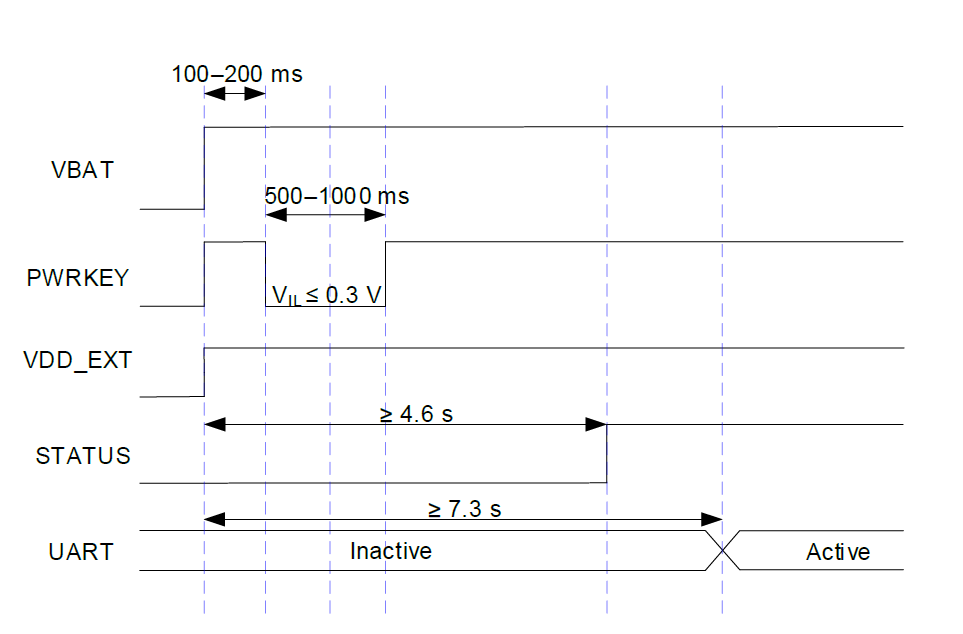
\includegraphics[width=0.8\columnwidth]{Slike/prizig_modula_BG955_HW_guide.png}
    \caption{Časovni diagram signalov ob prižigu modula}
    \label{prizig_modula_BG955_HW_guide}
\end{figure}
\newpage
Pin ima interni \SI{470}{\kilo\ohm} \textit{pull-up} upor. Ker konektor FEM po standardu P\textsuperscript{*} na svojem vmesniku nima za to namenjenega pina, smo zasnovali diskretno rešitev, ki jo prikazuje slika \ref{pwrkey}. Ob vklopu napajanja tranzistor PMOS Q103 ne prevaja, zato ne prevaja tudi tranzistor NMOS Q104 in je posledično signal \texttt{BG955\_PWRKEY} definiran z internim \textit{pull-up} uporom. Ko števec postavi signal \texttt{nRESET} v visoko stanje, tranzistor Q103 začne prevajati, kar povzroči polnjenje RC člena, sestavljenega iz upora R113 in kondenzatorja C115. Naloga prvega RC člena je zakasnitev pulza, drugi RC člen iz upora R115 ter kondenzatorja C117 pa se obnaša kot diferenciator, saj na vrata tranzistorja Q104 prenese zgolj spremembo vhodne napetosti, medtem ko se kondenzator C117 prazni prek upora R115. Ko je napetost med vrati in izvorom $U_{gs}$ tranzistorja Q104 večja od njegove pragovne napetosti $U_{GSth}$, se tranzistor odpre ter povzroči padec napetosti na liniji \texttt{BG955\_PWRKEY} na napetost \SI{0}{\volt}. 
Po preteku časovne konstante RC člena R115-C117 napetost na vratih tranzistorja pade pod pragovno napetost $U_{GSth}$, tranzistor Q104 preneha prevajati, linija \texttt{BG955\_PWRKEY} pa se zaradi internega pull-up upora ponovno postavi v logično visoko stanje. 
\begin{figure}[h]
    \centering
    \includesvg[inkscapelatex=false,width=0.95\columnwidth]{Slike/powerkey_vezje.svg}
    \caption{Vezje za avtomatski vklop modula}
    \label{pwrkey}
\end{figure}
\newpage
\section{Antena}
Antenski sklop omogoča, da lahko komunikacijski modul skupaj s števcem zanesljivo komunicira po brezžičnih omrežjih. Antena na komunikacijskem modulu mora podpirati več različnih frekvenčnih pasov, ki so navedeni v tabeli \ref{tab:bg955_bands}, frekvenčni spekter, v katerem bo antena delovala, pa prikazuje slika \ref{occupied_spectrum}. Iz slike lahko razberemo, da mora naša antena delovati v dveh frekvenčnih območjih od \SIrange{703}{960}{\mega\hertz} in od \SIrange{1710}{1880}{\mega\hertz}. Antenski sklop smo na predhodnih projektih načrtovali skupaj z podjetjem Ignion, ki nam je s simulacijami pomagalo določiti optimalen prostor ter prilagoditveno vezje za anteno. Izbrali smo linearno polarizirano čip anteno z enakomernim sevalnim diagramom, ki se jo na tiskano vezje pritrdi kot SMD komponento. Na njene lastnosti vplivajo številni dejavniki, med drugim oblika in dimenzije tiskanega vezja, geometrija ozemljitvene ravnine (angl. ground plane), bližina večjih kovinskih ali dielektričnih komponent ter nenazadnje tudi oblika in material ohišja.
\par Cilj pri načrtovanju prilagoditvenega vezja je impedanco antene v želenem frekvenčnem območju čim bolje prilagoditi impedanci komunikacijskega modula in karakteristični impedanci prenosne poti. V našem primeru je impedanca modula \SI{50}{\ohm}, za enako impedanco pa je načrtovana tudi prenosna pot. S tem zagotovimo, da se čim večji delež elektromagnetnega valovanja iz modula prenese na anteno in izseva v okolico ter obratno. Ključni parameter pri tem je koeficient odboja $\left|\Gamma\right|$, ki je definiran kot razmerje med odbito in vpadno amplitudo napetostnega vala. Iz njega lahko izpeljemo VSWR (tudi SWR) ter parametra $S_{11}$ oziroma Return\ Loss, ki to razmerje opisujeta v logaritemski skali. Razmerja med posameznimi parametri opisujejo enačbe \ref{Odbojni_parametri}.
\begin{equation} 
\begin{aligned}
|\Gamma|&=\frac{|V^-|}{|V^+|}  \\
\mathrm{SWR} &= \frac{1 + |\Gamma|}{1 - |\Gamma|} \\
S_{11}&=20\log_{10}\left(|\Gamma|\right) \\
\mathrm{Return\ Loss} &= -20\log_{10}\left(|\Gamma|\right) \\
\mathrm{Return\ Loss} &= -S_{11} 
\label{Odbojni_parametri}
\end{aligned}
\end{equation}

\begin{figure}[h]
    \centering
    \includesvg[inkscapelatex=false,width=0.95\columnwidth]{Slike/occupied_spectrum.svg}
    \caption{Frekvenčni spekter delovanja antene}
    \label{occupied_spectrum}
\end{figure}
\section{Kartica SIM}
Z variantno opremljenostjo smo zagotovili podporo klasične kartice SIM kot tudi eSIM. Obe različici uporabljata iste signale, ki jih opisuje standard ISO/IEC 7816-3:
\begin{description}[leftmargin=3cm,itemsep=0pt,topsep=0pt,parsep=0pt]
    \item \texttt{SIM\_VDD} -- napajanje kartice SIM je lahko \SI{1,8}{\volt} (razred C), \SI{3,3}{\volt} (razred B) ali \SI{5}{\volt} (razred A). BG955A-GL podpira kartice SIM razreda B in C, medtem ko se kartice razreda A praviloma ne uporabljajo več,
    \item \texttt{SIM\_DATA} -- dvosmerna komunikacija med modemom in kartico, ki je sinhronizirana s signalom SIM\_CLK. Amplituda je določena z razredom kartice SIM,
    \item \texttt{SIM\_CLK} -- ura, ki jo generira modem. Protokol uskladitve ure opisuje standard ETSI TS 102 221, maksimalna frekvenca ure pa je lahko \SI{26}{\mega\hertz},
     \item \texttt{SIM\_RST} -- reset kartice SIM. Napetostni nivo je določen z razredom kartice.
\end{description}
\par Med tipoma izbiramo s pomočjo \SI{0}{\ohm} uporov, ki preklopijo liniji \textit{CLK in DATA}. Pri izbiri fizične kartice SIM čim bližje nosilcu kartice dodamo ESD zaščito z nizko kapacitivnostjo, saj je nosilec kartice dostopen uporabniku.
\section{USB}
Povezava USB je na modul dodana z mislijo na dodatno razhroščevanje, vendar se med razvojem zaradi nepraktičnosti ni uporabljala. Za uporabo potrebujemo kabel TC2030-USB podjetja Tag-Connect, ki ima to prednost, da na samem modulu ne potrebujemo nobenega konektorja, ampak samo predpisan odtis (angl. footprint) na našem tiskanem vezju. Rešitev je primerna za tiskana vezja, kjer je na tiskanem vezju na voljo dovolj površine, v nasprotnem primeru pa nas lahko moti gostota lukenj, skozi katere ne moremo speljati vezi niti po vmesnih slojih. Zraven konektorja smo dodali ESD zaščito z nizko kapacitivnostjo. Pozornost smo namenili ustreznemu dimenzioniranju diferencialnih linij. Kabel in pripadajoč odtis prikazuje slika \ref{TC2030}.
\begin{figure}[h]
    \centering
    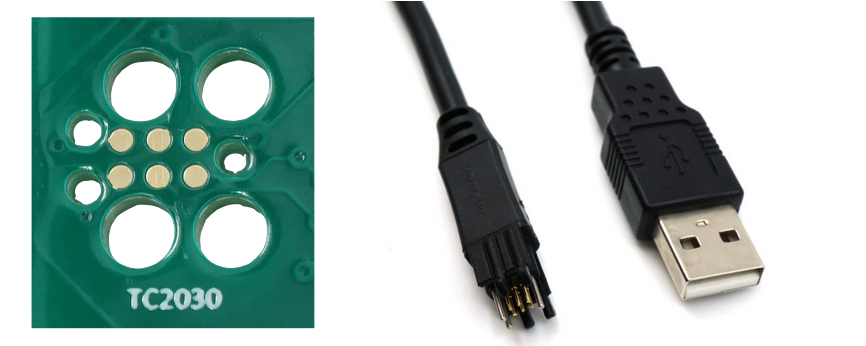
\includegraphics[width=0.8\columnwidth]{Slike/TC2030.png}
    \caption{Kabel TC2030-USB ter njegov odtis na tiskanem vezju}
    \label{TC2030}
\end{figure}


\section{Funkcija last gasp}
Ker je števec priklopljen na omrežje, mora biti vedno pripravljen na nenadni izklop. Števec detekcijo izpada napajanja opravlja na napetosti \SI{20}{\volt}, kot prikazuje slika \ref{blok_shema_napajanje_stevec}. Ob zaznanem izpadu se lahko (na števcih, ki to podpirajo) sproži funkcija \textit{last gasp}, katere namen je opozoriti distribucijsko podjetje s potisnim sporočilom, da je na omrežju prišlo do okvare oziroma izpada napajanja. Pogoj, da se funkcija izvede, je napolnjen ultrakondenzator. Glavni parametri funkcije so:
\begin{itemize}
    \item destinacija in način pošiljanja -- s tem parametrom nastavimo protokol in naslov IP potisnega sporočila,
    \item časovni interval ${t_f}$, po preteku katerega števec zaznani dogodek obravnava kot dejanski izpad napajanja (angl. power failure alarm filtering limit),
    \item največji naključni časovni zamik (angl. randomisation start interval) ${t_r}$ pred pošiljanjem potisnega sporočila. Ta preprečuje sočasno pošiljanje velikega števila sporočil z bližnjih števcev, kar bi lahko prekomerno obremenilo bazno postajo.
\end{itemize}

Med izpadom napajanja se števec in komunikacijski modul napajata iz ultrakondenzatorja, zato je treba za vse porabnike na števcu določiti, ali bodo v času izpada napajanja $t_{\mathrm{max}}$ prižgani, treba pa je tudi poskrbeti, da se mikrokrmilnik v števcu varno ustavi. 
Čas $t_{\mathrm{max}}$, ki ga določa enačba \ref{cas_last_gasp}, je omejen z velikostjo ultrakondenzatorja in je privzeto nastavljen na \SI{60}{\second}. Modul v času izvajanja funkcije ne dobi informacije, da je prišlo do izpada omrežja.
\begin{equation}
    t_{\mathrm{max}} > t_f + t_r 
    \label{cas_last_gasp} 
\end{equation}
    

\section{Varno ugašanje komunikacijskega modula}
Ko ultrakondenzatorju na števcu zmanjka naboja, se \SI{4}{\volt} napetost na števcu začne sesedati. Predhodno je bil edini način ugašanja modula BG955A-GL s signalom \texttt{PWRKEY} ali pa z ukazom AT, kar pa po podatkovnem listu lahko traja med \SIrange{650}{1500}{\milli\second}. Obstaja možnost, da bi med uporabo bliskovnega pomnilnika modulu odrezali napajanje, kar bi v skrajnih primerih lahko povzročilo okvaro pomnilnika. Tem okvaram se moramo v predpisani življenjski dobi števca (15 let) izogniti na vsak način, saj je zamenjava modula za distribucijo skrajno nezaželena. Skupaj s proizvajalcem modula smo prišli do rešitve, in sicer je Quectel implementiral t. i. funkcijo \textit{fastshutdown}.

\begin{figure}[h]
    \centering
    \includesvg[inkscapelatex=false, width=1\columnwidth]{Slike/fastshutdown_vezje.svg}
    \caption{Detektor padca napetosti}
    \label{fastshutdovn_vezje}
\end{figure}
Pin \texttt{GPIO6} na modulu ima definiran interni pull-up upor. Modul med delovanjem spremlja stanje pina in ob negativnem prehodu konča z vpisovanjem v bliskovni pomnilnik ter se ugasne. Vezje, ki ob padcu napetosti naredi negativni prehod na \texttt{GPIO6}, prikazuje slika \ref{fastshutdovn_vezje}.
Nadzornik napetosti NCP308 je med delovanjem števca napajan iz glavne napajalne žile za modul, ko pa števec modulu ugasne napajanje, se napaja iz kondenzatorja EDLC. Napetostni domeni smo ločili s Schottkyjevimi diodami, saj je poraba NCP308 zanemarljiva ter se posledično na njih ne izgublja veliko energije. Z delilnikom napetosti smo določili napetost, pri kateri NCP308 svoj \textit{open collector} izhod sklene na \SI{0}{\volt}. Izhod vezja ter delilnik napetosti smo povezali z \SI{1}{\mega\ohm} uporom in tako vezju dodali dodatno histerezo. Napetost preklopa ter histerezo določajo:
\begin{equation}
\begin{aligned}
   R_{100} &= \SI{8.25}{\kilo\ohm} \; (\pm1\,\%) \\ 
   R_{111} &= \SI{68.10}{\kilo\ohm} \; (\pm1\,\%) \\
   R_{117} &= \SI{1}{\mega\ohm} \; (\pm5\,\%) \\
    U_{\text{th}} &= \SI{0.405}{\volt}
\end{aligned}
\end{equation}
Tranzistorski izhod v NCP308 preneha prevajati, ko:
\begin{equation}
    U_{\text{sense}} \ge U_{\text{th}}
\end{equation}
Ob naraščajoči napajalni napetosti $U_{+4\mathrm{V}^\ast}$ je na izhodu NCP308 \SI{0}{\volt}:
\begin{equation}
    R_{100} \parallel R_{117} = \SI{8182.49}{\ohm}
\end{equation}
Izračunamo napetost $U_{\mathrm{TH}+}$ preklopa tranzistorja v NCP308:
\begin{equation}
\begin{aligned}
    U_{\mathrm{TH}+} &= \frac{U_{\text{th}}}{R_{100} \parallel R_{117}}\ \cdot R_{111} + U_{\text{th}} \\
    U_{\mathrm{TH}+} &= \frac{\SI{0.405}{\volt}}{\SI{8182,49}{\ohm}}\cdot \SI{68.1}{\kilo\ohm} + \SI{0.405}{\volt} \\
    U_{\mathrm{TH}+} &= \SI{3.78}{\volt}
\end{aligned}
\end{equation}
Tranzistorski izhod v NCP308 prične prevajati, ko:
\begin{equation}
    U_{\text{sense}} < U_{\text{th}}
\end{equation}
Ob padajoči napajalni napetosti $U_{+4\mathrm{V}^\ast}$ je na izhodu NCP308 \SI{4}{\volt}:
\begin{equation}
    R_{111} \parallel R_{117} = \SI{63758.1}{\ohm}
\end{equation}
Izračunamo napetost $U_{\mathrm{TH}-}$ preklopa tranzistorja v NCP308:
\begin{equation}
\begin{aligned}
    U_{\mathrm{TH}-} &= \frac{U_{\text{th}}}{R_{100}}\,\left(R_{111} \parallel R_{117}\right) + U_{\text{th}} \\
    U_{\mathrm{TH}-} &= \frac{\SI{0.405}{\volt}}{\SI{8250}{\ohm}}\cdot \left(\SI{68.1}{\kilo\ohm} \parallel \SI{1}{\mega\ohm}\right) + \SI{0.405}{\volt} \\
    U_{\mathrm{TH}-} &= \SI{3.53}{\volt}
\end{aligned}
\end{equation}

Ker je bila funkcija v začetnih verzijah implementacije slabo odzivna in nezanesljiva, smo modulu dodali zalogo energije v obliki kondenzatorja EDLC. Kondenzatorji tipa EDLC imajo veliko gostoto energije, nizek ESR ter lahko vzdržujejo velike tokove. Za prve vzorce smo izbrali kondenzator S06R0SA474WB proizvajalca Abracon, katerega ključne karakteristike so:
\begin{itemize}
    \item Kapacitivnost -- \SI{0,47}{\farad},
    \item Napetost -- \SI{6}{\volt},
    \item ESR -- \SI{0,9}{\ohm},
    \item Maksimalni tok -- \SI{1}{\ampere}.
\end{itemize}  

Da omejimo tok polnjenja, smo izbrali dva upora velikostnega razreda 1206 (v enačbah označena kot \textit{R1} in \textit{R2}) upornosti \SI{16}{\ohm}. Ta rešitev je bila izbrana, ker je cenovno ugodna in enostavna ob predpostavki, da montiran števec kondenzator EDLC napolni samo ob hladnem zagonu števca (ko je $U_{EDLC}$ = \SI{0}{\volt}), nato pa kondenzator ostane nabit med delovanjem števca.
Maksimalni polnilni tok kondenzatorja je:
\begin{equation} 
\begin{aligned}
    I_{max}&=\frac{U_0}{R1+R2} = \frac{\SI{4}{\volt}}{\SI{16}{\ohm}+\SI{16}{\ohm} }&= \SI{125}{\milli\ampere}
\end{aligned}
\end{equation}
Največjo moč na uporu \textit{R1} in \textit{R2} prikazuje enačba \ref{moc_upor}:
\begin{equation}
\begin{aligned}
    P_{R1_{max}}=P_{R2_{max}} &={I_{\max}}^2\cdot R\\
    \left(\SI{125}{\milli\ampere}\right)^2 \cdot \SI{16}{\ohm} &= \SI{0.25}{\watt}
    \label{moc_upor}
\end{aligned}
\end{equation}
Največja disipacija moči na uporih $P_{R1_{max}}$ in $P_{R2_{max}}$ nastopi v trenutku priklopa napajanja, ko je kondenzator popolnoma izpraznjen ($U_C$=\SI{0}{\volt}). V tem trenutku je polnilni tok največji, zato je največja tudi disipacija moči na uporih. Med polnjenjem kondenzatorja se njegova napetost povečuje, polnilni tok pa se eksponentno zmanjšuje, kar povzroči sorazmerno zmanjšanje disipirane moči na obeh uporih.
Minimalna napajalna napetost \SI{3,3}{\volt} bo na kondenzatorju dosežena približno ob času \SI{26,2}{\second}, kar prikazuje enačba \ref{polnjenje_EDLC}.
\begin{equation}
\begin{aligned}
    U_C(t)&=U_{Cmax}\left(1-e^{-t/\tau}\right) \\
    \tau &= R\cdot C \\
    \SI{32}{\ohm} \cdot \SI{0,47}{\farad} &= \SI{15.04}{\second} \\
    \SI{3,3}{\volt} &=\SI{4}{\volt}\left(1-e^{-t/\SI{15.04}{\second}}\right) \\
    t &\approx \SI{26,2}{\second} 
    \label{polnjenje_EDLC}
\end{aligned} 
\end{equation}
\par Da zalogo energije v kondenzatorju efektivno izkoristimo, moramo dodati vezje, ki bo ob izpadu napajanja premostilo polnilne upore, na katerih bi ob odjemu energije iz kondenzatorja dobili padec napetosti. To naredimo s tranzistorjem PMOS, ki mu vrata odpira kar napajalna napetost \SI{4}{\volt}, zato bo edina izguba predstavljala $R_{dsON}$ tranzistorja PMOS. Shemo prikazuje slika \ref{EDLC}.

\begin{figure}[h]
    \centering
    \includesvg[inkscapelatex=false, width=0.5\columnwidth]{Slike/EDLC.svg}
    \caption{Kondenzator EDLC za varno ugašanje modema}
    \label{EDLC}
\end{figure}
\newpage
\section{Načrtovanje tiskanega vezja}
Ko smo bili z rezultati simulacij in meritvami na prototipnih ploščah zadovoljni, smo narisali shemo in začeli načrtovati tiskano vezje. Vezje smo narisali v programu Altium Designer. Obliko tiskanega vezja, panel ter pozicijo konektorja smo imeli predhodno določeno. Odločili smo se za 4-slojno tiskanino, kjer je med prvim in drugim slojem \SI{0,18}{\milli\meter} razdalje, med drugim in tretjim \SI{1}{\milli\meter} ter med tretjim in četrtim slojem spet \SI{0,18}{\milli\meter}. Notranja sloja sta debela \SI{35}{\micro\meter}, zunanja pa sta zaradi postopka izdelave vezja debela do \SI{60}{\micro\meter}.
Komunikacijski modul in anteno smo postavili skupaj, da je linija, ki ju povezuje, ustrezno kratka. 
\newpage
Držali smo se naslednjih tehnoloških zahtev:
\begin{itemize}
    \item testne točke so na isti strani tiskanega vezja, da je proizvodno testiranje modula čim bolj dostopno, minimalna razdalja med njimi pa je \SI{2,54}{\milli\meter},
    \item vse SMD komponente so opremljene na eni strani, ni pa nam tega uspelo zagotoviti za THT komponente, saj kondenzatorja EDLC nismo mogli prestaviti na drugo stran zaradi omejitve z višino ohišja,
    \item v okolici konektorja in kondenzatorja smo pustili dovolj prostora za postopek selektivnega spajkanja,
    \item vezje smo ustrezno označili s fiducialnimi oznakami.
\end{itemize}
Pri načrtovanju smo upoštevali:
\begin{itemize}
    \item na prvem notranjem sloju nismo naredili nobenih povezav z razlogom, da čim manj prekinjamo ozemljitveno ravnino, ki je direktno pod komponentami,
    \item linije, po katerih teče tok, ki napaja komunikacijski modul, so dovolj debele, da na njih ni napetostnega padca,
    \item med linijami, ki povezujejo kartico SIM z modulom, smo pustili razmak, da ne bi zaradi hitrih prehodov napetosti prišlo do presluha,
    \item ESD zaščite smo postavili čim bližje viru potencialne motnje.
\end{itemize}
Sloje tiskanega vezja prikazuje slika \ref{TIV}.
\begin{figure}[h] 
\centering 
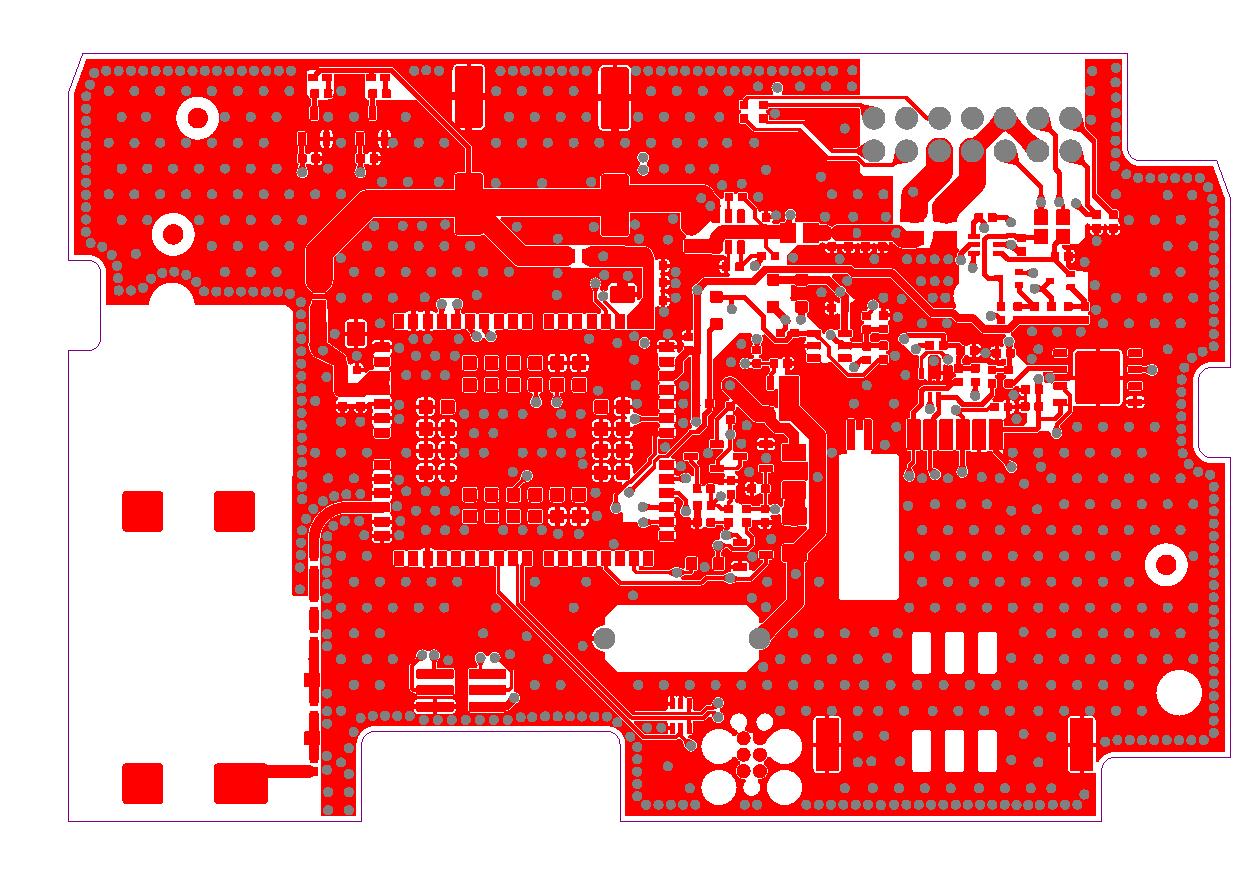
\includegraphics[page=1, width=0.7\textwidth,angle=90]{Slike/layerli_mag.pdf}\hfill
\includegraphics[page=2, width=0.7\textwidth,angle=90]{Slike/layerli_mag.pdf} \vspace{2mm} 
\includegraphics[page=3, width=0.7\textwidth,angle=90]{Slike/layerli_mag.pdf}\hfill 
\includegraphics[page=4, width=0.7\textwidth,angle=90]{Slike/layerli_mag.pdf} 
\caption{Sloji tiskanega vezja} 
\label{TIV} 
\end{figure}
\newpage

  
%Oscilogram napetostne pretvobe na RX liniji Main UART prikazuje slika ref{Napetostni pretvornik}.
%\begin{figure}[h]
%    \centering
%    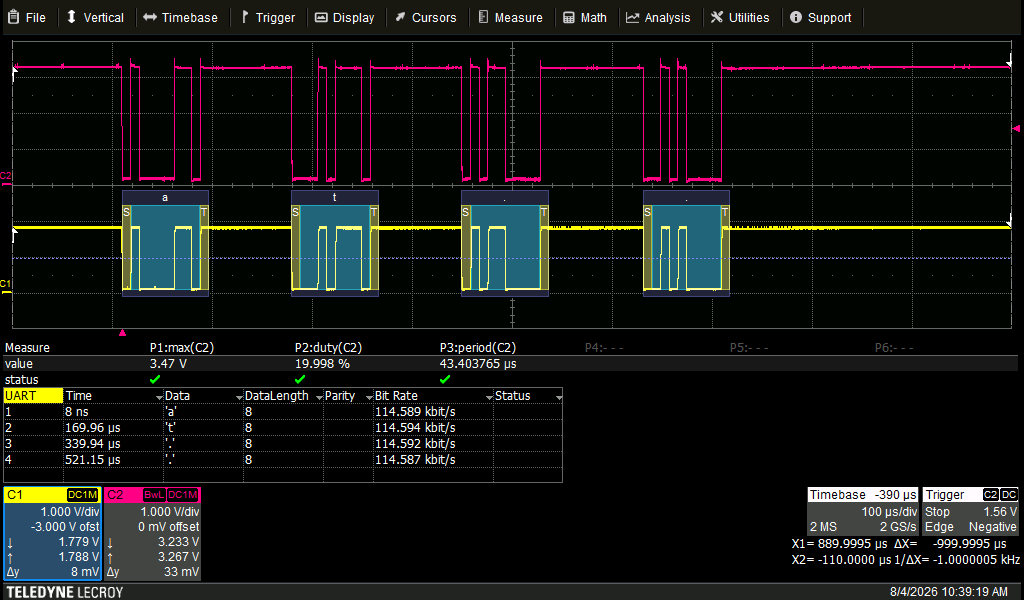
\includegraphics[width=0.9\columnwidth,trim=0cm 0.4cm 0.0cm 0.8cm, clip]{Slike/moduleRX level translator.PNG}
%    \caption{Napetostni pretvornik med 3.3V in 1.8V}
%    \label{Napetostni pretvornik}
%\end{figure}

%, rezultat na samem vezju pa prikazuje slika \ref{Negativni_pulz_pwrkey}
%\begin{figure}[h]
%    \centering
%    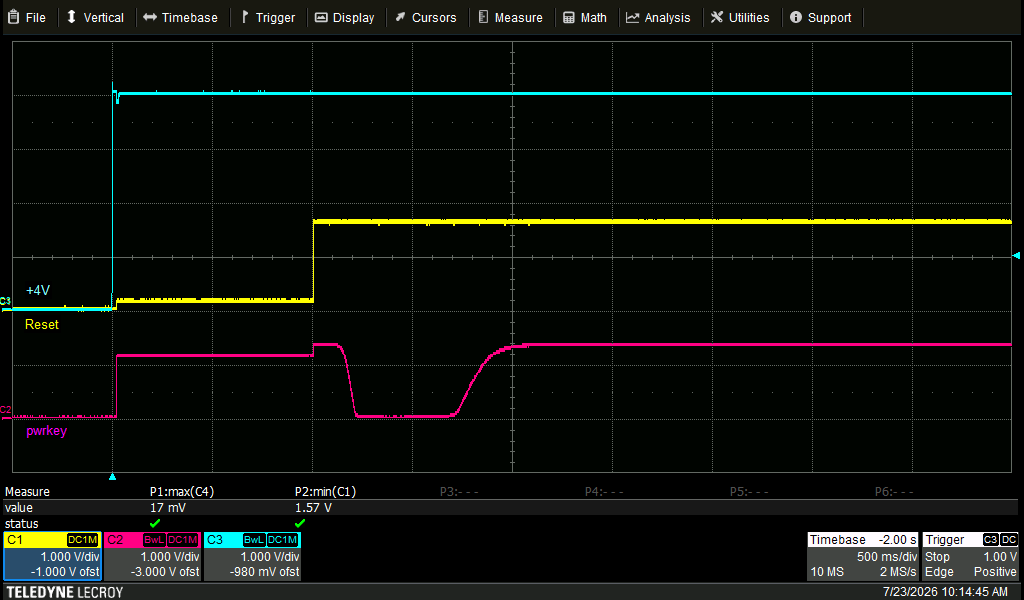
\includegraphics[width=0.9\columnwidth,trim=0cm 0.4cm 0.0cm 0.8cm, clip]{Slike/vklop.PNG}
%    \caption{Negativni pulz na signalu \texttt{BG\_955\_PWRKEY}}
%    \label{Negativni_pulz_pwrkey}
%\end{figure}
\chapter{Testiranje komunikacijskega modula}
Načrtovano tiskano vezje smo naročili ter ga opremili v proizvodnji podjetja. Izdelek je prikazan na sliki \ref{modul}. Sledilo je testiranje, pri katerem smo poudarek namenili funkcijskim sklopom, opisanim v zgornjih poglavjih. Pri testiranju smo si pomagali z interno razvito vgrajeno programsko opremo ADT (Advanced Test Bench), namenjeno razvojnemu in proizvodnemu testiranju. Omogoča nam testiranje strojne opreme in uporabo določenih delov periferije (GPIO, UART, SPI ipd.) mikrokrmilnika na števcu. 
\begin{figure}[!h]
    \centering
    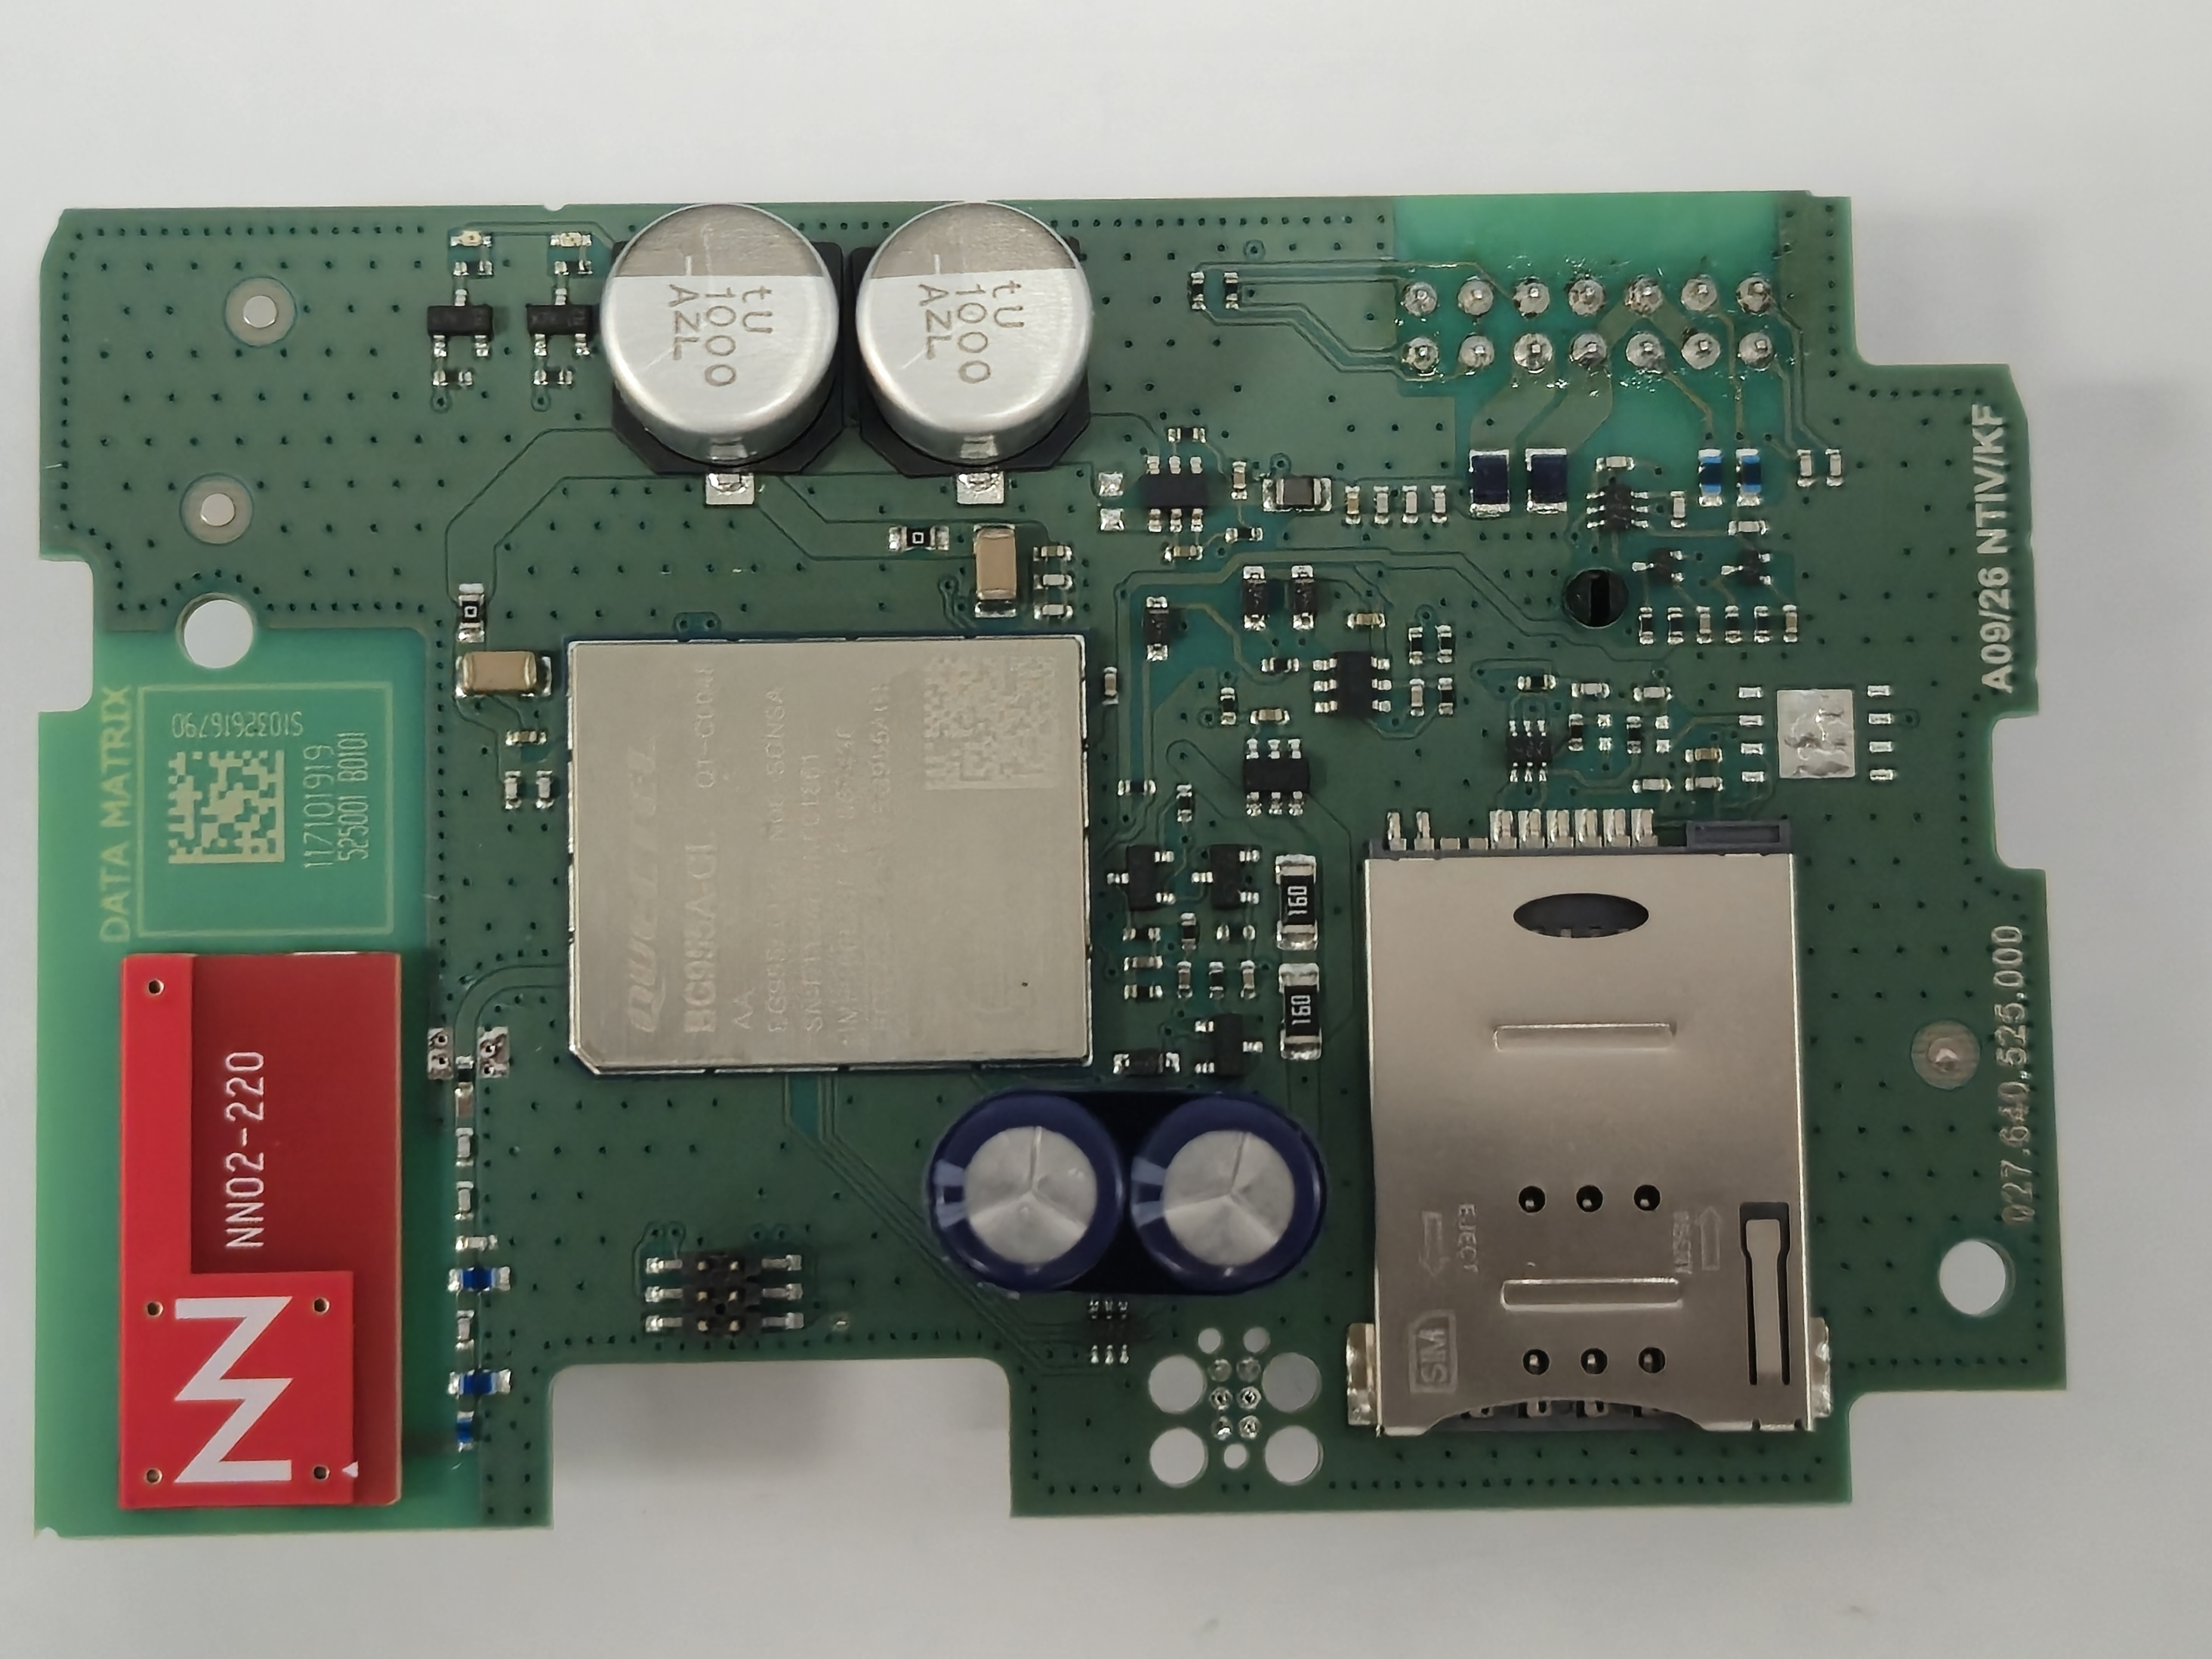
\includegraphics[width=0.6\columnwidth,angle=270,trim=0cm 5cm 8cm 10cm, clip]{Slike/modul2.jpg}%
    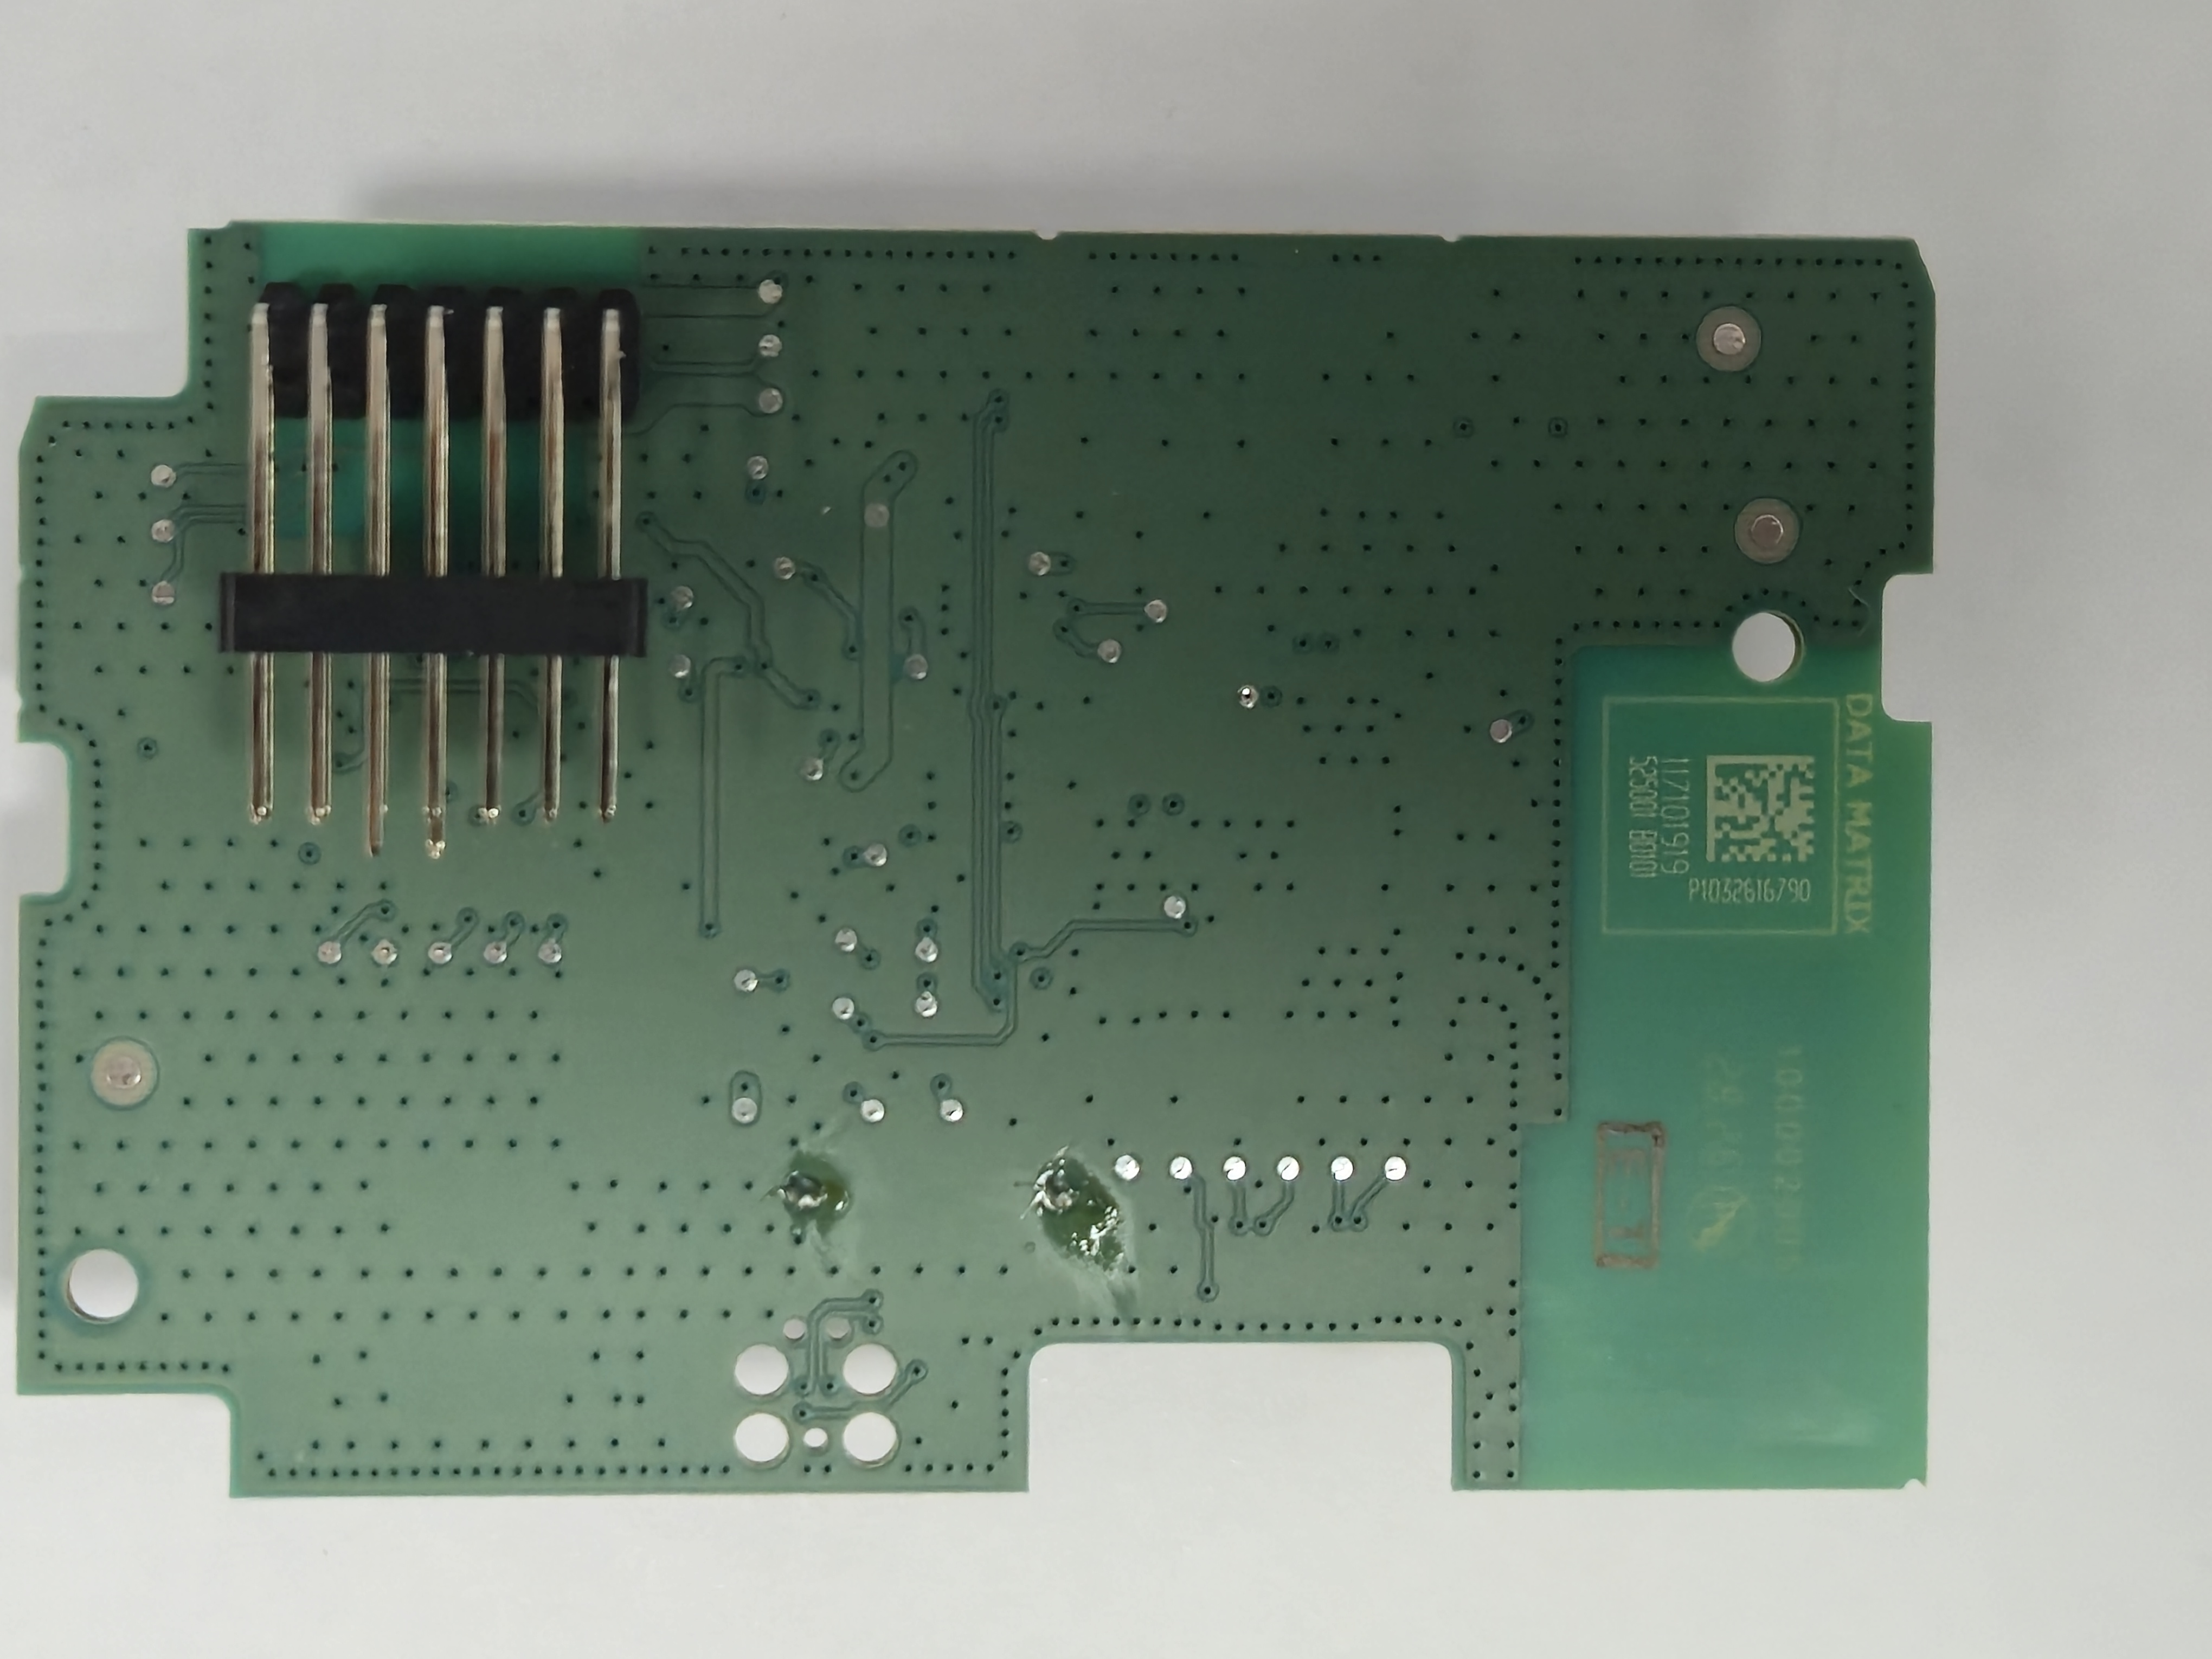
\includegraphics[width=0.6\columnwidth,angle=270,trim=0cm 10cm 12cm 12cm, clip]{Slike/modul1.jpg}
    \caption{Izdelan komunikacijski modul}
    \label{modul}
\end{figure}
\section{Vklop modula}
Pri vklopu modema BG955 smo opazili, da je napetost na pinu \texttt{PWRKEY} nižja, kot smo pričakovali (\SI{1,8}{\volt}). Najprej smo za to okrivili tok puščanja tranzistorja NMOS (\SI{1}{\micro\ampere}) v kombinaciji z velikim notranjim \textit{pull-up} uporom (\SI{470}{\kilo\ohm}). Ob odstranitvi tranzistorja smo ugotovili, da napetost ostaja ista, torej že sam modul generira napetost, nižjo od \SI{1,8}{\volt}. Položne prehode na liniji si razlagamo z zelo majhnim tokom \textit{Id} skozi tranzistor in posledično širokim območjem napetosti \textit{Ug}, pri katerem tranzistor še prevaja ta tok. Prižig modula prikazuje slika \ref{Negativni_pulz_pwrkey}.
\begin{figure}[!h]
    \centering
    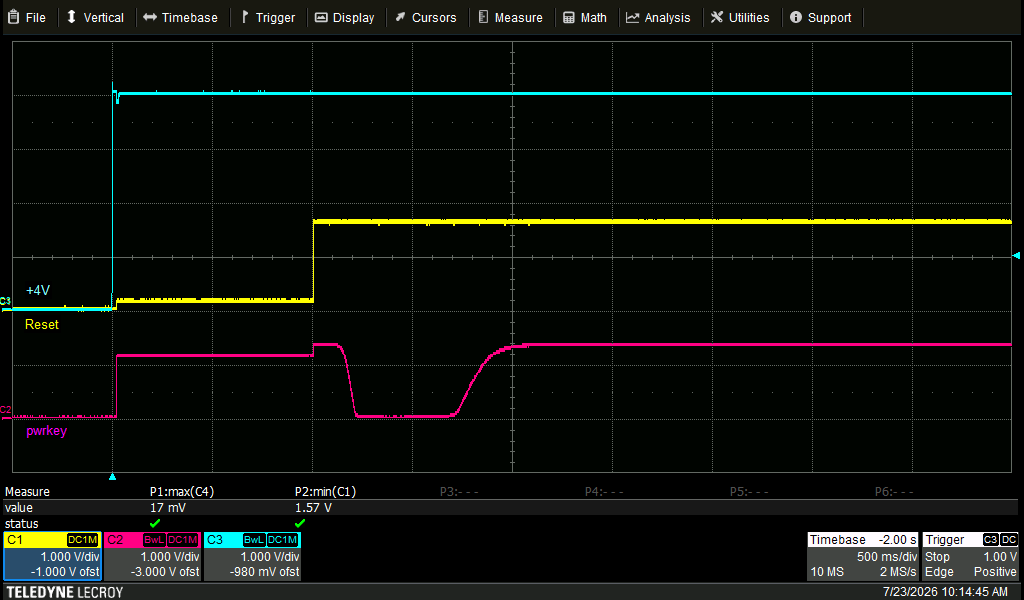
\includegraphics[width=0.9\columnwidth,trim=0cm 0.4cm 0.0cm 0.8cm, clip]{Slike/vklop.PNG}
    \caption{Negativni pulz na signalu \texttt{BG955\_PWRKEY}}
    \label{Negativni_pulz_pwrkey}
    \vspace{5pt}
    \small
    \begin{tabular}{@{}ll@{}}
        Opis signalov na oscilogramu:\\
        Modra: &glavna napajalna napetost modula (\SI{4}{\volt}) \\
         Rumena: &napetost na pinu \texttt{nRESET} \\
         Magenta:   & napetost na pinu \texttt{PWRKEY} \\
    \end{tabular}
\end{figure}

\section{Napetostni pretvornik za UART}
Diskretni pretvornik napetosti je deloval, kot smo si zamislili, vendar pa smo pri testiranju opazili počasne napetostne prehode v smeri iz modula proti števcu. Razlog smo našli v kondenzatorjih, ki so na števčni strani konektorja FEM nameščeni zaradi elektromagnetne kompatibilnosti. Kapacitivnost teh kondenzatorjev glede na tip števca variira med \SI{33}{\pico\farad} in \SI{270}{\pico\farad}, ob hitrih prehodih signala \texttt{UART TX} pa lahko v kombinaciji z \SI{10}{\kilo\ohm} \textit{pull-up} upori povzročijo položne pozitivne prehode. Kljub temu da je pri funkcijskem testu komunikacija potekala normalno, smo se odločili vezje narediti bolj robustno z zamenjavo obstoječih \textit{pull-up} uporov z manjšimi \SI{1}{\kilo\ohm} upori.

\section{Testiranje napajanja}
\par Z elektronskim bremenom smo testirali delovanje tokovne limite. Na glavno napajalno linijo smo z merilnimi vezmi povezali elektronsko breme in nastavili tok na \SI{2}{\ampere}. Slika \ref{fig:tokovna_limita} prikazuje, kako se \SI{4}{\volt} napetost na števcu minimalno posede, napetost na modulu pa sesede. Tokovna limita se zaradi toka skozi njo ter razlike napetosti med vhodom in izhodom segreje in posledično prekine tok, ki teče skoznjo, dokler se ne ohladi dovolj. 
\begin{figure}[!h]
    \centering
    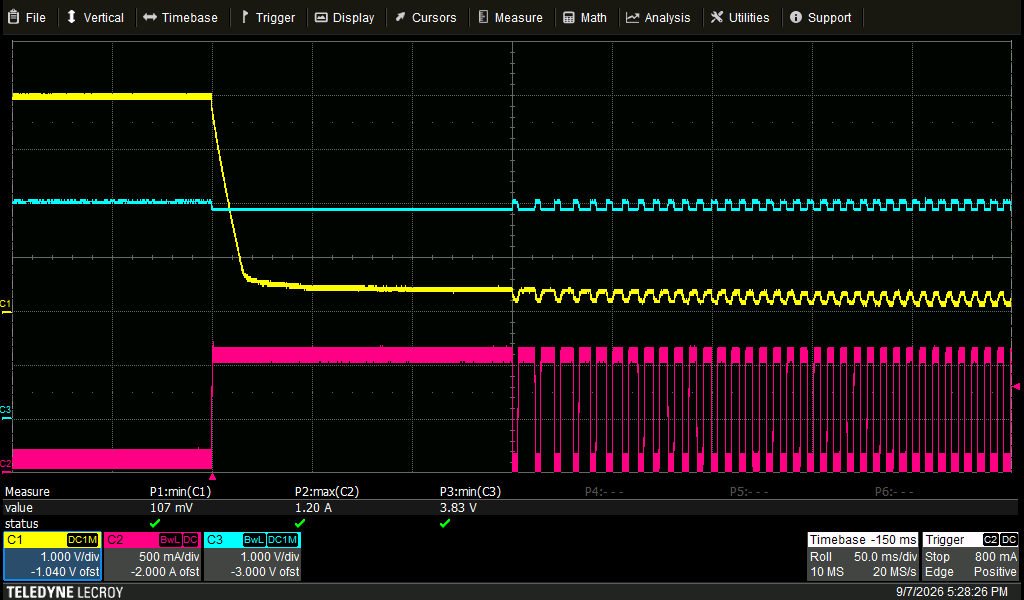
\includegraphics[width=0.9\columnwidth,trim=0cm 0.4cm 0.0cm 0.8cm, clip]{Slike/tokovna_limita2.png}
    \caption{Odziv tokovne limite}
    \label{fig:tokovna_limita}
    \vspace{5pt}
    \small
    \begin{tabular}{@{}ll@{}}
         Opis signalov na oscilogramu:\\
         Rumena: &glavna napajalna napetost modula (\SI{4}{\volt}) \\
         Modra:      & \SI{4}{\volt} napetostna linija na števcu \\
         Magenta:   & tok, ki teče iz števca v modul \\
    \end{tabular}
\end{figure}
\par
Modul, opremljen s kartico SIM, se je po ustrezni konfiguraciji APN-ja in konteksta PDP uspešno povezal v mobilno omrežje ter pridobil naslov IP. Po vzpostavitvi povezave modul preklopimo v način delovanja GPRS in prek konzole svojega osebnega računalnika izvajamo ukaz ping proti modemu ter opazujemo napajalno napetost modema. Na sliki \ref{GPRS_power_dip} lahko vidimo, da se napetost ob t. i. TX burstu posede, vendar ne pod kritično mejo, ki je definirana v podatkovnem listu modema. Opazili smo, da je tok iz števca v modul manjši od tokovne limite \SI{1}{\ampere}, kar bo treba nadalje raziskati, verjetno pa je manjši tok posledica feritnih dušilk na števcu in modulu, ki so namenjene zmanjševanju visokofrekvenčnih motenj na napajanju. Slika prikazuje porabo toka ter posedanje napetosti na glavni napajalni liniji. 
\begin{figure}[!h]
    \centering
    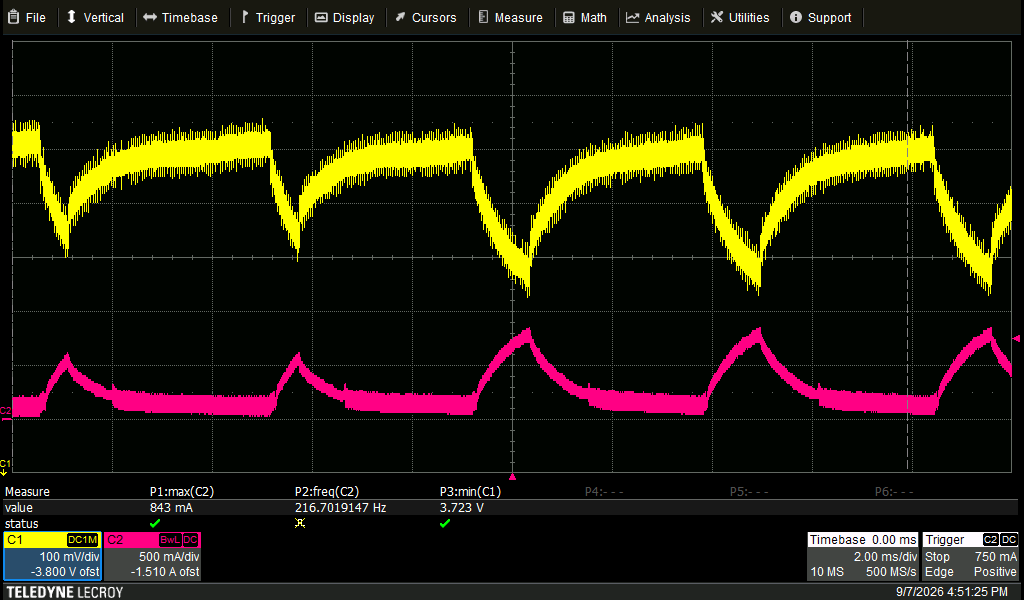
\includegraphics[width=0.9\columnwidth,trim=0cm 0.4cm 0.0cm 0.8cm, clip]{Slike/GPRS burst3.png}
    \caption{Posedanje napetosti na napajalni liniji med komunikacijo GPRS}
    \label{GPRS_power_dip}
    \vspace{10pt}
    \small
    \begin{tabular}{@{}ll@{}}
        Opis signalov na oscilogramu:\\
         Rumena: &glavna napajalna napetost modula (\SI{4}{\volt}) \\
         Magenta:   & tok, ki teče iz števca v modul \\
    \end{tabular}
\end{figure}
\par
Preverili smo tudi delovanje funkcije \textit{last gasp}. Ultrakondenzator na števcu je napolnjen na napetost \SI{2}{\volt}, ob izpadu napajanja pa s pomočjo navzgornjega pretvornika (angl. boost converter) napetost na ultrakondenzatorju dvignemo na \SI{4}{\volt}. Blokovno shemo prikazuje slika \ref{blok_shema_napajanje_stevec}. Pretvornik navzgor svojo funkcijo opravlja, dokler je napetost na ultrakondenzatorju vsaj \SI{0,5}{\volt}. Števcu smo nastavili parametra časovni interval ${t_f}$ in največji naključni časovni zamik ${t_r}$ na \SI{30}{\second}, zato pričakujemo, da števec pošlje sporočilo v času med \SI{30}{\second} in \SI{60}{\second} po izpadu napajanja na izbrani naslov IP ter vrata prek protokola UDP. Na računalniku smo spremljali komunikacijo na določenih vratih in uspešno prejeli števčevo sporočilo, ob tem pa smo na osciloskopu spremljali napetost na števčnem kondenzatorju. Rezultat testa je oscilogram na sliki \ref{last_gasp}, kjer lahko iz oblike toka razberemo, da je števec sporočilo poslal po približno \SI{52}{\second} in da je v ultrakondenzatorju še dovolj energije za varno ugašanje števca.
\begin{figure}[!h]
    \centering
    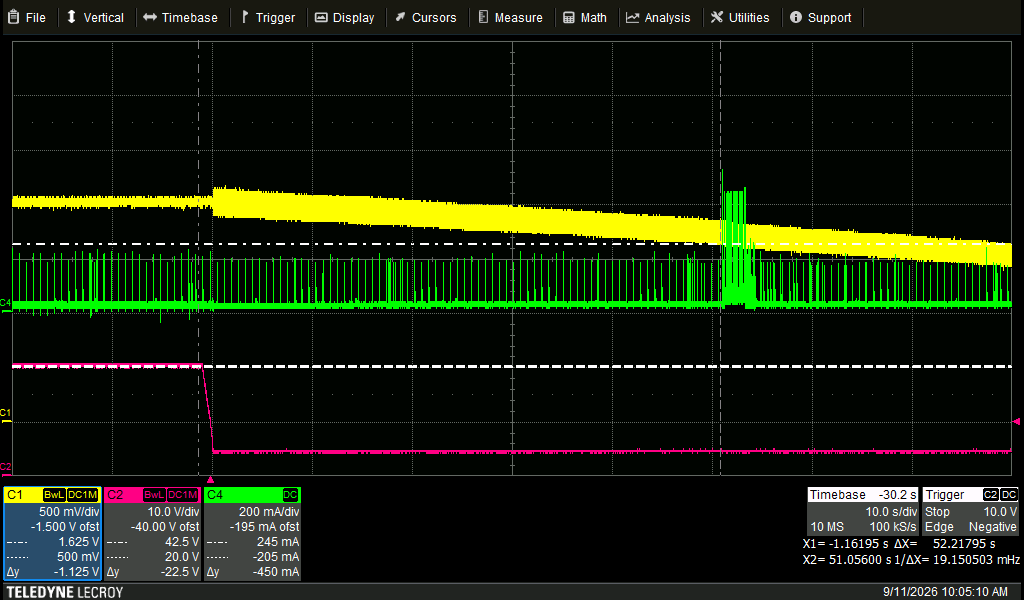
\includegraphics[width=0.9\columnwidth,trim=0cm 0.4cm 0.0cm 0.8cm, clip]{Slike/last gasp.png}
    \caption{Praznenje ultrakondenzatorja na števcu po izpadu napajanja}
    \label{last_gasp}
    \vspace{10pt}
    \small
    \begin{tabular}{@{}ll@{}}
        Opis signalov na oscilogramu:\\
         Rumena: &napetost na ultrakondenzatorju \\
         Magenta:   &\SI{20}{\volt} linija na števcu, na kateri se opravlja detekcija \\
         &izpada napajanja \\
         Zelena:   &tok, ki teče iz števca v modul
    \end{tabular}
\end{figure}

\newpage
\section{Antenski sklop}
Meritev antene smo opravili z vektorskim analizatorjem omrežij. S tiskanega vezja smo odstranili modem in na njegovo mesto prispajkali konektor U.FL. Nato smo modul vstavili v števec ter ga zaprli s pokrovom, na katerega smo priklopili ustrezno kalibriran vektorski analizator, s katerim smo izmerili parameter SWR. Na sliki \ref{VNA} vidimo, da imamo v frekvenčnih območjih od približno \SIrange{700}{760}{\mega\hertz} in \SIrange{1700}{1760}{\mega\hertz} \( \mathrm{SWR} > 3 \) (oziroma \SI{6}{\decibel} Return Loss), kar kaže na slabo impedančno prilagoditev antene v tem frekvenčnem območju. Naredili smo prve popravke ter mejno zadostili kriteriju \( \mathrm{SWR} < 3 \). 

\begin{figure}[h] 
\centering 
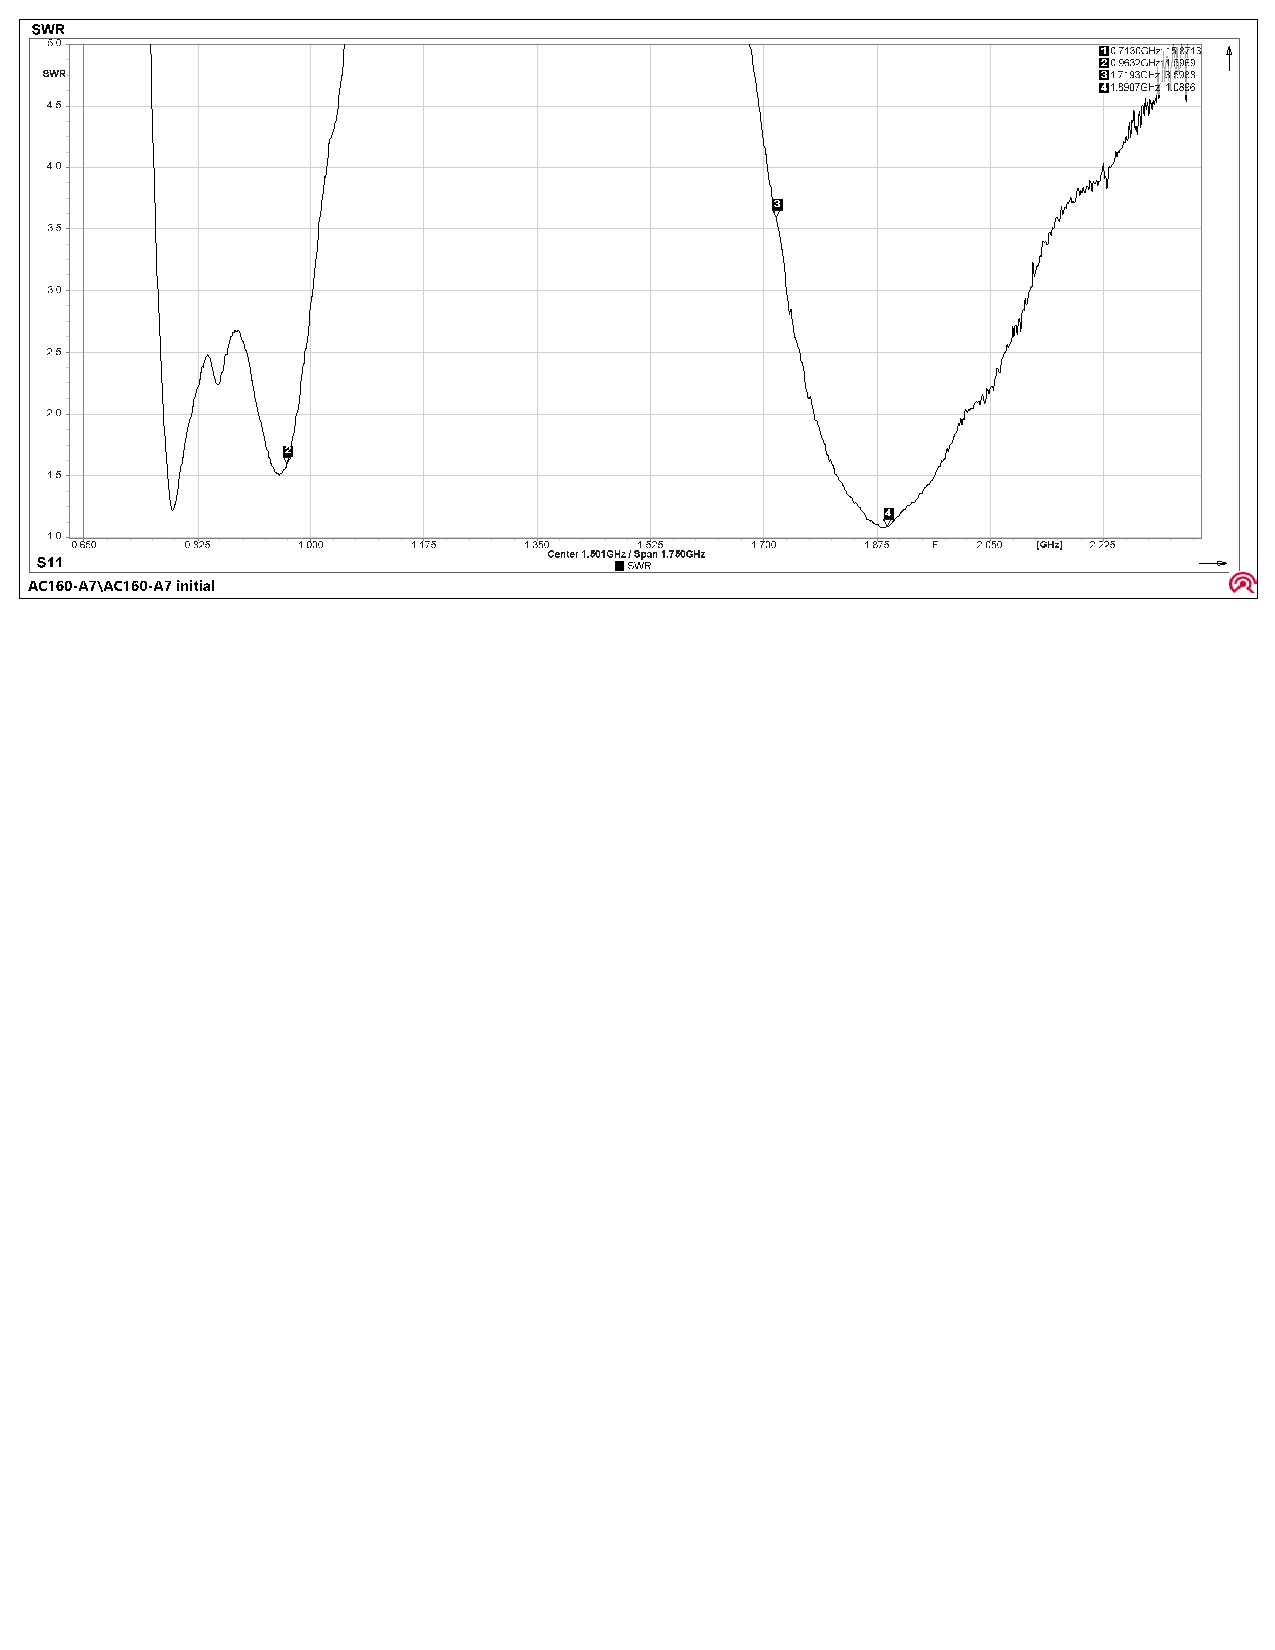
\includegraphics[width=0.8\columnwidth,trim=0cm 17.0cm 0cm 0.0cm, clip]{Slike/VNA_original.pdf} 
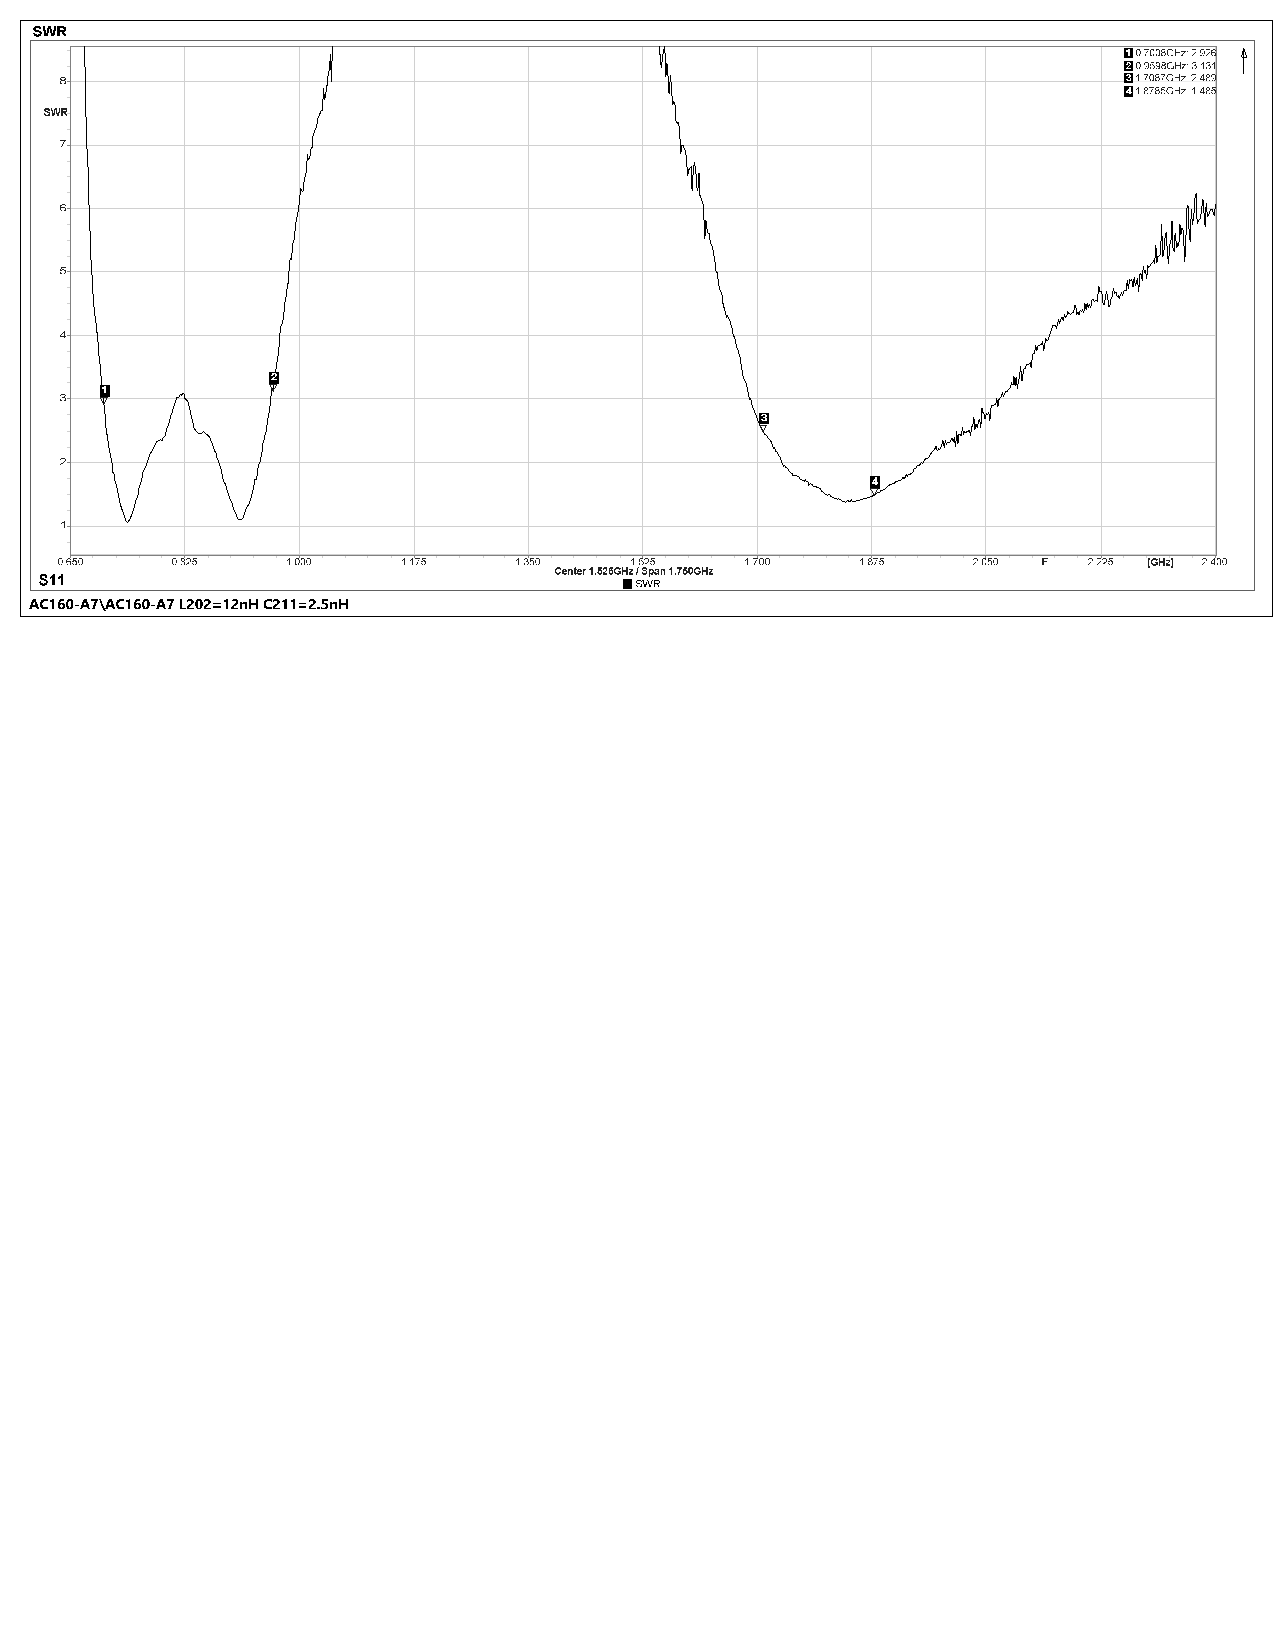
\includegraphics[width=0.79\columnwidth,trim=0cm 17.0cm 0cm 0.0cm, clip]{Slike/VNA_popravek.pdf} 
\caption{Meritev SWR s prvotno impedančno prilagoditvijo (zgornja slika) in po prvem popravku (spodnja slika)} 
\label{VNA} 
\end{figure}
Z modulom, vgrajenim v števec, smo izvedli meritve OTA. Pri teh meritvah sta nas zanimala parametra TRP in TIS. 

\par TRP predstavlja skupno moč, ki jo komunikacijska naprava izseva v prostor v vseh smereh. Parameter je definiran kot integral prostorske porazdelitve izsevane moči po celotnem prostorskem kotu in predstavlja merilo oddajne učinkovitosti celotnega sistema. Med meritvijo je komunikacijski modul nastavljen v način neprekinjenega oddajanja, pri čemer se izsevana moč meri v zaporednih prostorskih točkah okoli naprave. Na podlagi tako pridobljenih meritev se z ustreznim prostorskim povprečenjem določi vrednost parametra TRP.

\par TIS predstavlja povprečno sprejemno občutljivost sistema po celotnem prostorskem kotu in podaja najmanjšo moč sprejetega signala, pri kateri sistem še zagotavlja predpisano kakovost sprejema oziroma zahtevano vrednost bitne napake (BER). Meritev poteka podobno kot pri določanju parametra TRP, le da se v tem primeru meri občutljivost sprejemnika. Na vrednost TIS poleg antene in njene prilagoditve pomembno vpliva tudi delovanje same naprave, saj se lahko elektromagnetne motnje, ki jih ustvarja naprava, sklopijo na anteno in s tem poslabšajo sprejemno občutljivost sistema. Oba parametra sta izražena v enoti dBm ter sta močno odvisna od sevalnega diagrama uporabljene antene. 

Merilno postavitev sestavljajo:
\begin{itemize}
    \item predcertifikacijska OTA-komora Minilab \SI{6}{\giga\hertz} za meritve TRP in TIS,
    \item tester radijskih komunikacij Rohde \& Schwarz CMW500,
    \item računalnik, ki krmili CMW500 in komoro prek omrežne povezave.
\end{itemize}
\par Meritve smo izvedli le s prvo iteracijo filtra, nato pa je komora zaradi nepričakovane okvare potrebovala servis. Merjeni števec je imel naloženo vgrajeno programsko opremo ADT, zato rezultati TIS niso popolnoma veljavni, saj med meritvijo večina periferije števca ni delovala ter posledično ni proizvajala motenj. Pri parametru TIS smo zaradi dolgotrajnega postopka merili samo sredinske kanale, pri TRP pa smo izmerili spodnji, sredinski in zgornji kanal ter tako pokrili večino frekvenčnega spektra posameznega pasu. Rezultate prikazuje tabela \ref{tab:trp_tis_results}. Iz njih lahko razberemo zadovoljivo delovanje antenskega sklopa, z izjemo frekvenčnega pasu B28, kjer so rezultati slabi, kar je glede na impedančno prilagoditev na tem frekvenčnem spektru pričakovano. Rezultat TRP v obliki sevalnega diagrama prikazuje slika \ref{TRP}.

\begin{footnotesize}
\begin{table}[H]
    \centering
    \caption{\label{tab:trp_tis_results} Rezultati meritev TRP in TIS za tehnologijo LTE Cat-M}
    ~\\*
    \setlength{\tabcolsep}{4pt}
    \begin{tabular}{
        @{}
        c
        S[table-format=5.0]
        S[table-format=4.2]
        S[table-format=2.2]
        @{\hspace{1.5em}}
        c
        S[table-format=4.0]
        S[table-format=4.2]
        S[table-format=-3.2]
        @{}
    }
       \hline 
        \multicolumn{4}{c}{\rule{0pt}{3ex}\textbf{TRP}} &
        \multicolumn{4}{c}{\textbf{TIS}} \\[0.5ex]
        \hline
        \rule{0pt}{3ex}
        \textbf{Pas} &
        \multicolumn{1}{c}{\textbf{Kanal}} &
        \multicolumn{1}{c}{\textbf{Frekvenca}} &
        \multicolumn{1}{c}{\textbf{TRP}} &
        \textbf{Pas} &
        \multicolumn{1}{c}{\textbf{Kanal}} &
        \multicolumn{1}{c}{\textbf{Frekvenca}} &
        \multicolumn{1}{c}{\textbf{TIS}} \\
        &
        &
        \multicolumn{1}{c}{\textbf{[MHz]}} &
        \multicolumn{1}{c}{\textbf{[dBm]}} &
        &
        &
        \multicolumn{1}{c}{\textbf{[MHz]}} &
        \multicolumn{1}{c}{\textbf{[dBm]}} \\[0.5ex]
        \hline
        B3  & 19225 & 1710.52 & 18.79 & B3  & 1575 & 1844.03 & -104.45 \\
        B3  & 19575 & 1747.86 & 19.66 & B8  & 3625 &  943.94 & -102.11 \\
        B3  & 19925 & 1784.48 & 20.64 & B20 & 6300 &  807.44 &  -98.31 \\
        B8  & 21475 &  880.52 & 19.19 & B28 & 9435 &  776.54 &  -97.13 \\
        B8  & 21625 &  897.86 & 19.35 &     &      &         &         \\
        B8  & 21775 &  914.48 & 18.96 &     &      &         &         \\
        B20 & 24175 &  832.52 & 18.79 &     &      &         &         \\
        B20 & 24300 &  847.36 & 18.91 &     &      &         &         \\
        B20 & 24425 &  861.48 & 19.47 &     &      &         &         \\
        B28 & 27235 &  703.52 &  7.24 &     &      &         &         \\
        B28 & 27435 &  723.52 & 11.12 &     &      &         &         \\
        B28 & 27635 &  743.52 & 12.98 &     &      &         &         \\
        \hline
    \end{tabular}
\end{table}
\end{footnotesize}

\begin{figure}[h] 
\centering 
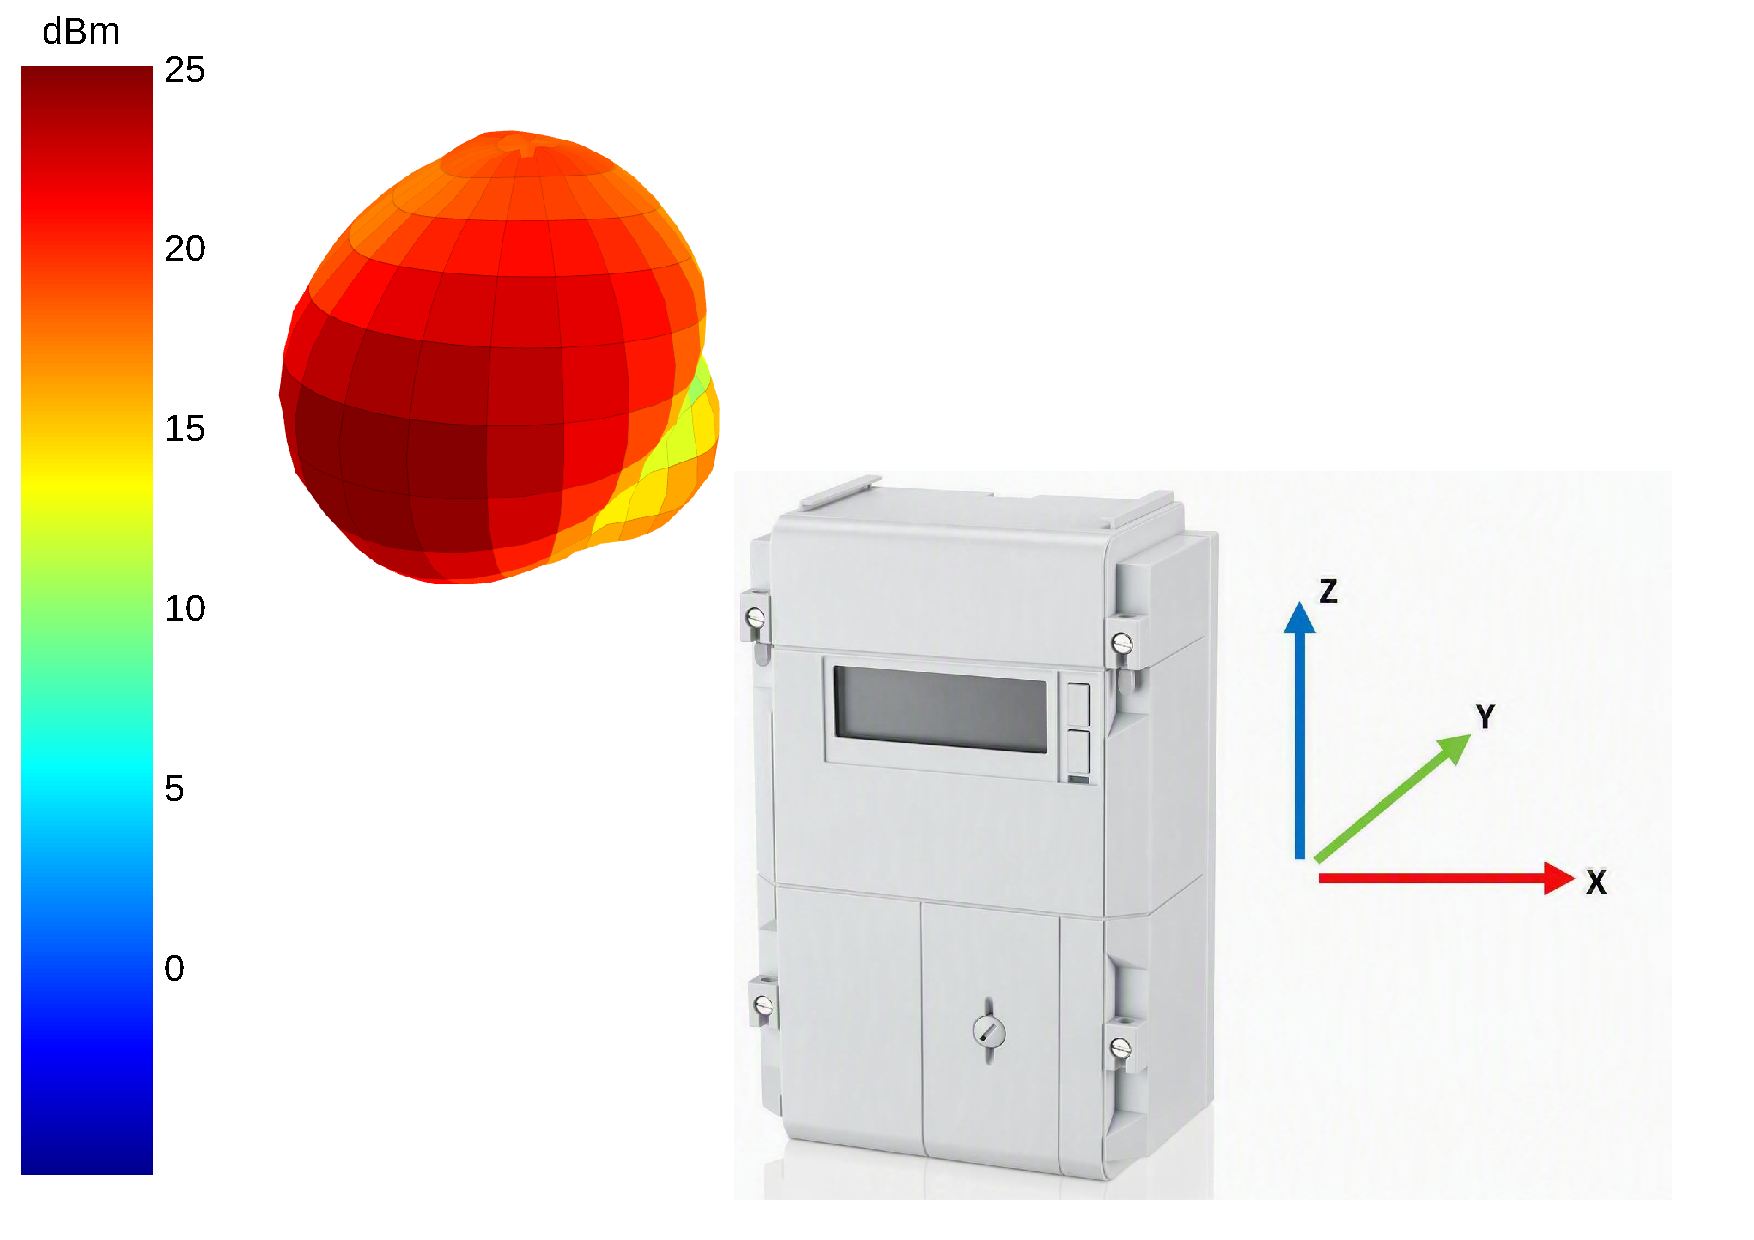
\includegraphics[width=0.8\columnwidth,trim=0cm 0.0cm 0cm 0.0cm, clip]{Slike/band 8 mid chanel trp.pdf} 
\caption{Sevalni diagram TRP v tehnologiji LTE Cat-M, Band 8, kanal 21475} 
\label{TRP} 
\end{figure}
\newpage
\section{Hitra ustavitev modula}
Ob povezavi v omrežje smo lahko testirali funkcijo \textit{fastshutdown}. Modul smo priklopili na nastavljiv napetostni izvir ter pomerili napetosti, pri katerih preklopi NCP308. Histerezo prikazuje slika \ref{fig:fastshutdown_detektor_oscilogram}, s pomočjo markerjev lahko odčitamo, da sta napetosti $U_{TH-}$ in $U_{TH+}$ \SI{3.49}{\volt} in \SI{3.82}{\volt}, kar se ujema z izračuni v prejšnjem poglavju, manjša odstopanja pa pripisujemo tolerancam komponent.

\begin{figure}[!h]
    \centering
    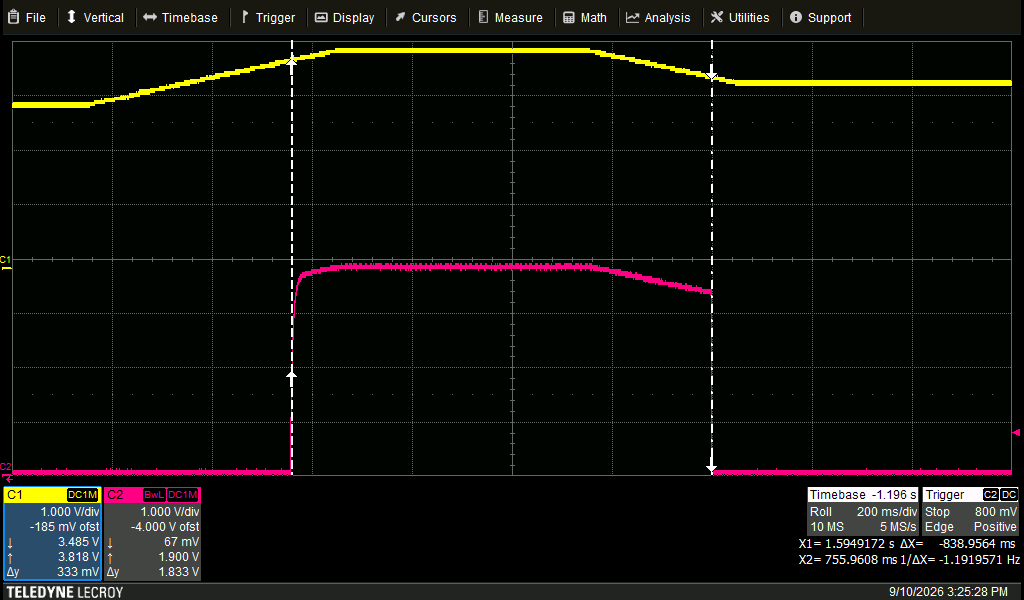
\includegraphics[width=0.9\columnwidth,trim=0cm 0.4cm 0.0cm 0.8cm, clip]{Slike/fastshutdown_detektor.png}
    \caption{Histereza preklopa nadzornika napetosti NCP308}
    \label{fig:fastshutdown_detektor_oscilogram}
    \vspace{10pt}
    \small
    \begin{tabular}{@{}ll@{}}
         Opis signalov na oscilogramu:\\
         Rumena: &glavna napajalna napetost modula (\SI{4}{\volt}) \\
         Modra:      &napetost na \texttt{nRESET} pinu nadzornika napetosti NCP308 \\
    \end{tabular}
\end{figure}

Ker nismo imeli točnih informacij o implementaciji te funkcije, smo predpostavili, da modul v bliskovni pomnilnik vpisuje podatke ob zagonu ter ob povezavi v omrežje. V programskem jeziku Python smo napisali skripto, ki krmili števec z naloženim ADT, preverja odziv modula na \textit{debug UART} ter prek omrežja iz osciloskopa odčitava čas, ki ga je modem potreboval, da se je ugasnil, kar signalizira z ugasnitvijo statusne diode LED. Isti signal ter signal, na katerem se zgodi negativni prehod, ki narekuje izvedbo funkcije \textit{fastshutdown}, opazujemo z osciloskopom, na katerem predhodno nastavimo, da nam ob vsaki sproženi meritvi prebere časovno razliko med obema padajočima signaloma ter jo shrani, nato pa podatek preberemo z osebnim računalnikom. Potek skripte prikazuje slika \ref{testna_skripta}. 
\begin{figure}[h]
    \centering
    \includesvg[inkscapelatex=false, width=0.5\columnwidth]{Slike/Testna_skripta.svg}
    \caption{Blokovna shema skripte za testiranje funkcije \textit{fastshutdown}}
    \label{testna_skripta}
\end{figure}

\begin{figure}[h]
    \centering
    \includesvg[inkscapelatex=false, width=0.7\columnwidth]{Slike/rezultati_fastshutdown.svg} \vspace{2mm} 
    \includesvg[inkscapelatex=false, width=0.7\columnwidth]{Slike/rezultati_fastshutdown2.svg}
    \caption{Primerjava dveh verzij funkcije \textit{fastshutdown}, zgoraj starejša, spodaj novejša, optimizirana verzija}
    \label{rezultati}
\end{figure}


V obdobju razvoja komunikacijskega modula je Quectel izdal novo verzijo programske opreme, ki je vsebovala popravke za funkcijo \textit{fastshutdown}, zato smo lahko primerjali rezultate, kar prikazuje slika \ref{rezultati}. Vidimo, da so bili popravki učinkoviti, saj se je čas ugašanja modula skrajšal na stotino prvotne vrednosti.




\chapter{Zaključek}
V magistrskem delu smo predstavili celoten potek načrtovanja, razvoja in testiranja komunikacijskega modula za družino pametnih števcev IE.X podjetja Iskraemeco. Izhajajoč iz zahtev internega standarda P\textsuperscript{*} smo zasnovali modul, ki temelji na modemu BG955A-GL proizvajalca Quectel in podpira tehnologije LTE Cat-M, NB-IoT ter GPRS.

V okviru razvoja smo obravnavali ključne funkcijske sklope modula. Razložili smo diskretni pretvornik napetostnih nivojev med \SI{3,3}{\volt} in \SI{1,8}{\volt} logiko, vezje za samodejni vklop modula z zakasnjenim generiranjem negativnega pulza na pinu \texttt{PWRKEY} in napajalni del s tokovno limito, ki preprečuje prevelik odjem toka iz števca. Pozornost smo namenili zanesljivemu delovanju ob izpadu napajanja in varnemu ugašanju modema, skupaj s proizvajalcem uvedli funkcijo hitrega izklopa (\textit{fastshutdown}) ter zasnovali strojni prožilnik te funkcije, dopolnjen z dodatno zalogo energije v kondenzatorju, ki preprečuje okvaro bliskovnega pomnilnika ob nenadni prekinitvi napajanja. Na koncu smo modul realizirali na 4-slojnem tiskanem vezju, ki smo ga načrtovali v skladu s pravili EMC ter zahtevami za proizvodno testiranje.

 Potrdili smo pravilno delovanje tokovne limite in pretvornika napetostnih nivojev, pri čemer smo naleteli na izziv, saj je bilo delovanje pretvornika napetostnih nivojev odvisno tudi od števca, na katerega nismo imeli vpliva. Z vektorskim analizatorjem omrežij smo izmerili impedančno prilagoditev antene ter po popravkih prilagoditvenega vezja dosegli kriterij $\mathrm{SWR} < 3$ v frekvenčnem območju delovanja antene. V predcertifikacijski komori smo izvedli meritve izsevane moči (TRP) in sprejemne občutljivosti (TIS), ki so pokazale solidno delovanje antenskega sklopa v večini frekvenčnih pasov, razen v frekvenčnem pasu B28. 
 
 Razvili smo avtomatiziran postopek za testiranje funkcije \textit{fastshutdown}, ki nam bo tudi v prihodnosti pomagal pri testiranju robnih pogojev, ki se pojavljajo ob nenadnih izklopih. S tem postopkom smo ovrednotili izboljšavo funkcije \textit{fastshutdown} po nadgradnji vgrajene programske opreme. Glede na rezultate testiranja funkcije \textit{fastshutdown} bodo potrebne ponovne meritve, ki nam bodo povedale, ali je shranjevanje dodatne energije v kondenzatorju EDLC sploh potrebno.

Pri delu smo se soočili tudi z omejitvami. Prva je bila nepričakovana okvara predcertifikacijske komore, zaradi katere nam je uspelo izvesti le meritve s prvo iteracijo antenskega filtra. Druga pa je bila uporaba testne programske opreme (ADT), saj v času testiranja še nismo imeli števčne vgrajene programske opreme, ki bi podpirala naš modem. Posledično rezultati TIS niso povsem reprezentativni, saj med meritvijo večina periferije števca ni delovala in zato ni proizvajala elektromagnetnih motenj. Pri analiziranju rezultatov smo opazili korelacijo med slabo impedančno prilagoditvijo antene in radijskimi zmogljivostmi komunikacijskega modula. Zaradi zasedenosti laboratorija EMC v podjetju še nismo testirali elektromagnetne skladnosti modula v kombinaciji s števcem.

Da bo modul dokončno industrializiran, nas čaka še nekaj iteracij impedančne prilagoditve antene, ponovno merjenje v predcertifikacijski komori, testiranje doslej še neodobrenih komponent ter validacijsko testiranje, pri katerem se bodo preverile vse funkcije števca, ki uporabljajo komunikacijski modul in jih sami nismo preverili.
\cleardoublepage\phantomsection\addcontentsline{toc}{chapter}{Literatura} % vnos literature v kazalo
% 1. način: BibTeX
\bibliographystyle{./Izgled/ieeetrslo}
\bibliography{literatura}

\end{document}
%%%%%%%%%%%%%%%%%%%%%%%%%%%%%%%%%%%%%%%%%%%%%%%%%%%%%%%%%%%%%%%%%%%%%%%%%%%%%%%%%%%%%%%%%%%%%%%%%%%%%%%%%%%%%%%%%%%%%%%%
